%%%%%%%% Technical memo, 11-25-2026: cross-entropy versus correlation for AI judges %%%%%%%%%
% ICML 2026 style, preprint option. Build: `make` in this directory (pdflatex + bibtex).
% Every number in the text is printed by a committed script under ../../experiments/ or by make_memo_assets.py;
% provenance comments (% Provenance:) sit beside each block of numbers.

\documentclass{article}

\usepackage{microtype}
\usepackage{graphicx}
\usepackage{subcaption}
\usepackage{booktabs}
\usepackage{longtable}
\usepackage{hyperref}
\newcommand{\theHalgorithm}{\arabic{algorithm}}

\usepackage[preprint]{icml2026}

\usepackage{amsmath}
\usepackage{amssymb}
\usepackage{mathtools}
\usepackage{amsthm}
\usepackage[capitalize,noabbrev]{cleveref}

\theoremstyle{plain}
\newtheorem{proposition}{Proposition}[section]
\newtheorem{lemma}[proposition]{Lemma}
\theoremstyle{remark}
\newtheorem{remark}[proposition]{Remark}

% The memo is dated by hand: the preprint footer prints \today.
\renewcommand{\today}{November 25, 2026}

\newcommand{\RPS}{\mathrm{RPS}}
\newcommand{\CE}{\mathrm{CE}}
\newcommand{\TVD}{\mathrm{TVD}}
\newcommand{\KL}{\mathrm{KL}}
\newcommand{\E}{\mathbb{E}}
\newcommand{\Var}{\operatorname{Var}}
\newcommand{\Cov}{\operatorname{Cov}}
\newcommand{\Ind}{\mathbf{1}}
\newcommand{\appref}[1]{Appendix~\ref{#1}}
\newcommand{\expref}[1]{experiment~#1}

\icmltitlerunning{Cross-Entropy, Not Correlation, for AI Judges}

\begin{document}

\twocolumn[
  \icmltitle{Learn Judges Like Any Other Model: Cross-Entropy, Not Correlation,\\
    for Predicting Human Rating Distributions}

  \icmlsetsymbol{equal}{*}

  \begin{icmlauthorlist}
    \icmlauthor{Brando Miranda}{stanford}
  \end{icmlauthorlist}

  \icmlaffiliation{stanford}{Department of Computer Science, Stanford University, Stanford, CA, USA}
  \icmlcorrespondingauthor{Brando Miranda}{brando9@stanford.edu}

  \icmlkeywords{LLM-as-a-judge, proper scoring rules, ranked probability score, cross-entropy, evaluation, scaling laws}

  \vskip 0.3in
]

\printAffiliationsAndNotice{}
\setlength{\textfloatsep}{14pt plus 2pt minus 4pt}
\setlength{\dbltextfloatsep}{14pt plus 2pt minus 4pt}
\setlength{\floatsep}{10pt plus 2pt minus 2pt}
\setlength{\dblfloatsep}{10pt plus 2pt minus 2pt}
\setlength{\intextsep}{10pt plus 2pt minus 2pt}

\begin{abstract}
Teams validate AI judges by their correlation with human ratings.
Correlation sees only conditional means, and only up to a positive affine map.
It cannot tell a judge with the right means and the wrong rating distributions from a correct one.
We treat a judge as a probability model of human ratings, fit it with cross-entropy and score it with proper scores, chiefly the ranked probability score (RPS).
An exact three-item example matches every conditional mean, so Pearson correlation is 1, yet it has mean total variation distance 0.20 and cross-entropy 1.065 against 0.915 nats.
Across synthetic targets and human ratings of theorems, homework, images, dialogue, helpfulness and inference, cross-entropy fitting usually beats Pearson fitting on held-out RPS (lower is better); SummEval summaries are the exception, where at 768 ratings the cross-entropy fit selects the uniform forecast (RPS 0.284) and the Pearson fit scores 0.144.
Frozen frontier judges with a calibration head cross over at 4--8 ratings, one per item, in all 25 judge-by-dataset cells.
Matched low-rank adaptation (LoRA) of Qwen3-4B and Llama-3.1-8B favors cross-entropy in all seven setups at the largest budget, by 0.013 to 0.076 RPS on raw forecasts and 0.0002 to 0.0043 after one shared calibration.
A saturating power law fits the held-out RPS curve of cross-entropy-fit judges in 9 of 11 panels (median exponent 0.66 on RPS and 0.82 on cross-entropy where the floor is identified) and that of Pearson-fit judges in 1 of 11 (exponent 0.09, extrapolated floor).
Correlation remains competitive below about eight ratings, when the mean barely varies, and for choosing a single judge from some pools.
Judges are an ordinary supervised learning problem: choose a proper loss, hold out data and fit the learning curve.
\end{abstract}

\section{Introduction}
\label{sec:intro}

Teams validate AI judges at scale by their correlation with human ratings~\citep{liu2023geval,zheng2023judging}.
Pearson correlation measures the linear association between the judge's scores and human ratings, and rank correlations measure agreement in order.
Neither says whether the judge predicts how experts rate each input.
That distinction matters whenever a decision uses probabilities, thresholds or averages of the judge's output.

We model the judge as a conditional distribution.
Given an item $x$ (a problem, a candidate answer, a reference), expert ratings $r\in\{0,\dots,K-1\}$ vary across raters and occasions.
We write $p(r\mid x)$ for that distribution and $q(r\mid x)$ for the judge's forecast.
Fitting $q$ is ordinary supervised learning with a proper loss, and evaluating it is forecast verification~\citep{gneiting2007strictly}.
This memo supports the blog post that makes this argument~\citep{miranda2026bitter}, in the spirit of the bitter lesson~\citep{sutton2019bitter}: use the general method, give it data and measure how error falls with data.

Correlation cannot identify $p$.
Pearson correlation across items depends on a forecast only through its conditional means, and only up to a positive affine map.
On $K$ categories, $K-2$ shape directions per item stay free, and so do the level and the scale of the means (Section~\ref{sec:identification}, \appref{app:proofs}, \appref{app:moments}).
Identification does not settle the matter, because a flexible model trained on correlation can still land on the right distribution.
We therefore ask an empirical question.
How many human ratings does a cross-entropy-fitted judge need before it beats a correlation-fitted judge on held-out ratings, and does the answer survive across datasets, models and objectives?

This memo consolidates every experiment in the repository (30 active folders and four archived ones, numbered 00--33; \appref{app:index}) and builds on the identification preprint~\citep{miranda2026correlation}.
We make five contributions.
\begin{enumerate}
\item \textbf{Identification.} We prove what Pearson correlation, mean squared error, cross-entropy and the ranked probability score identify, bound moment recovery by cross-entropy, and give an exact three-item example with equal means and different distributions (Section~\ref{sec:identification}; derivations in \appref{app:moments}).
\item \textbf{Controlled studies.} On synthetic ratings with known distributions, cross-entropy training beats Pearson training from 12 ratings when the mean carries the signal (experiment 08, three ratings per task) and from 48 in a second toy whose spread and shape also vary (experiment 20, where it loses at 12).
When the mean says little, it needs 192 ratings against Pearson, Spearman and mixed objectives and 24 against Kendall (experiment 06, scenario A; Section~\ref{sec:controlled}).
\item \textbf{Frozen judges on human ratings.} With five frontier judges and a 27-setting calibration head, cross-entropy fitting clears Pearson fitting and a uniform forecast after 4--8 ratings, one per item, in all 25 dataset-by-judge cells of ChaosNLI and DICES (Section~\ref{sec:frozen}).
\item \textbf{Trained judges.} In matched LoRA fine-tuning with four objectives, Pearson-trained judges have higher raw RPS than CE-trained judges in all seven setups at the largest budget.
Squared error and CE differ by $0.0003$ RPS at $K=2$ (interval includes zero), and CE beats squared error on five of six panels with $K\ge3$ (Section~\ref{sec:lora}).
\item \textbf{Scaling laws.} A floor plus $aN^{-b}$ fits the held-out RPS curves of cross-entropy-fit judges in 9 of 11 panels (median $b=0.66$ where the floor is identified) and those of Pearson-fit judges in 1 of 11 (Section~\ref{sec:scaling}).
\end{enumerate}

\paragraph{Related work.}
\citet{han2025judgesverdict} report, across 54 judges, that high correlation with humans does not guarantee human-like agreement.
\citet{guerdan2025validating} show that validating judges against forced-choice human labels can select judges performing as much as 31\% worse than selection that accounts for rating indeterminacy.
\citet{elangovan2025beyond} show that one aggregate correlation can hide differences when human labels are uncertain.
We add training and a matched-budget comparison of objectives.

\section{Setting, objectives and metrics}
\label{sec:setting}

\paragraph{Data and units.}
Item $x_i$ has human distribution $p_i$ over ratings $r\in\{0,\dots,K-1\}$ and mean $t_i=\sum_r r\,p_i(r)$.
A judge forecast $q_i$ has mean $m_i=\sum_r r\,q_i(r)$.
A training budget $N$ is the total number of individual human ratings spent on fitting.
It can sit on $N$ items with one rating each ($d=1$ rating per item) or on $N/d$ items with $d$ ratings each.
Test scores average over held-out items, and each held-out item is scored against all of its collected ratings.

\paragraph{Objectives.}
Pearson fitting maximizes the correlation between forecast means and the mean training rating of each item.
Cross-entropy (CE) fitting minimizes $-\log q_i(r_{ij})$ averaged over individual training ratings.
RPS fitting and mean squared error (MSE) fitting minimize the squared cumulative-probability gap and the squared error $(m_i-r_{ij})^2$ on the same ratings (\appref{app:protocols}).
For a frozen judge, a fit chooses among 27 calibration settings of the judge's own probabilities $p$,
\begin{equation}
q\;\propto\;p^{\,t}\exp\!\bigl(b\,u_k+c\,u_k^{2}\bigr),
\label{eq:head}
\end{equation}
with $t\in\{\tfrac12,1,2\}$, $b,c\in\{-1,0,1\}$ and $u_k$ the centered, scaled category index.
Search is exhaustive; ties go to the setting nearest the identity; every objective sees the same settings and the same training ratings.
For a trained judge, LoRA weights~\citep{hu2022lora} and a probability read-out are updated by each objective under one optimizer, one schedule and one validation rule.

\paragraph{Metrics.}
The primary metric is the normalized individual-rating ranked probability score,
\begin{equation}
\RPS(q,r)=\frac{1}{K-1}\sum_{k=0}^{K-2}\bigl(F_q(k)-\Ind\{r\le k\}\bigr)^2 ,
\label{eq:rps}
\end{equation}
where $F_q$ is the cumulative distribution of $q$.
It lies in $[0,1]$, lower is better, and it is strictly proper~\citep{epstein1969scoring,gneiting2007strictly}.
We pair it with CE in nats (lower is better) and with total variation distance $\TVD=\tfrac12\sum_r|h(r)-q(r)|$ to each item's empirical human distribution $h$, averaged equally over items.
TVD is a diagnostic of the whole distribution, not a proper score for individual ratings.
Every table lists reference forecasts: a uniform forecast, the judge's raw output, and where relevant the training histogram.
Pearson, Spearman and Kendall correlations are secondary diagnostics of ranking.

\paragraph{Differences, uncertainty and break-even.}
A difference always subtracts the same metric on the same data for two named procedures.
We write it in words, for example ``test RPS of the Pearson-fitted judge minus test RPS of the CE-fitted judge'', and positive values favor CE.
Intervals are bootstraps over held-out items (over prompts for HelpSteer2, over folds with an overlap-adjusted $t$ interval for the homework studies), with simultaneous max-$t$ bands across budgets where stated; draws and levels are listed per experiment in \appref{app:protocols}.
The break-even budget $N^\ast$ is the smallest budget from which the lower bound for ``Pearson-fit minus CE-fit'' and for ``uniform minus CE-fit'' both stay above zero at every larger budget tested.
Selection of a fitted judge is by training data (and validation data where stated), never by the test ratings.

\section{What correlation can and cannot identify}
\label{sec:identification}

Fix $n\ge2$ items with true rating distributions $P_i$ on $\{0,\dots,K-1\}$, item means $t_i$, forecasts $q_i$ and forecast means $m_i$.
Pearson correlation across items is $\rho(m,t)=\sum_i(m_i-\bar m)(t_i-\bar t)/(n\,s_m s_t)$ and is undefined when either vector is constant.
All statements below are proved in \appref{app:proofs}; they restate the identification preprint~\citep{miranda2026correlation} with the cross-entropy (CE), ranked probability score (RPS) and Pearson definitions of Section~\ref{sec:setting}.

\begin{proposition}[Pearson sees means up to a positive affine map]
\label{prop:affine}
For nonconstant $m$ and $t$, forecasts with equal item means have equal correlation, $\rho(a\mathbf 1+bm,t)=\rho(m,t)$ for every $a\in\mathbb R$ and $b>0$, and $\rho(m,t)=1$ if and only if $m=a\mathbf 1+bt$ for some $a\in\mathbb R$, $b>0$.
\end{proposition}

The statement concerns the output, not the model.
A neural judge may map inputs to means by any nonlinear function and still reach $\rho=1$; Pearson measures the linear association between predicted and human ratings, and does not make the judge linear.

\begin{proposition}[Unidentified directions]
\label{prop:dimension}
For $K=2$ a forecast is fixed by its mean, so correlation one leaves only the level $a$ and scale $b$.
For $K\ge3$ the distributions with a fixed interior mean form a set of dimension $K-2$, and the all-positive set of forecasts with correlation one has dimension $n(K-2)+2$.
\end{proposition}

Binary ratings therefore remove the shape ambiguity and keep the level and scale ambiguity.
For $K=2$ and correlation-one means $m_i=a+bt_i$, the excess expected RPS is $n^{-1}\sum_i(a+(b-1)t_i)^2$, which is zero only at $a=0$, $b=1$.
Three or more categories add $K-2$ free shape directions per item.

\begin{proposition}[What each objective identifies]
\label{prop:losses}
(i) Mean squared error satisfies $\E[(a-R)^2\mid x]=(a-t(x))^2+\Var(R\mid x)$, so it identifies the conditional mean and nothing else.
(ii) $\CE(P,q)=H(P)+\KL(P\|q)$, so CE is uniquely minimized by $q=P$.
(iii) With $d_k=F_P(k)-F_q(k)$, $\bar d$ their average and $m_q,m_P$ the two means, the excess expected RPS is
\begin{equation}
\mathcal E_P(q)=\frac{(m_q-m_P)^2}{(K-1)^2}+\frac1{K-1}\sum_{k=0}^{K-2}(d_k-\bar d)^2 ,
\label{eq:rps-decomp}
\end{equation}
which vanishes only at $q=P$, and $|m_q-m_P|\le(K-1)\TVD(P,q)$.
\end{proposition}

Equation~\eqref{eq:rps-decomp} shows what RPS adds to a mean: the first term is the mean error, the second is everything else in the cumulative distribution, and it is the only term that remains when the means agree.
Total variation distance to the true distribution is zero only at $q=P$ but is not a proper score for individual ratings (\appref{app:proofs}), which is why we report it as a diagnostic.

\begin{proposition}[CE controls every bounded moment]
\label{prop:moments}
For $m_j(q,x)=\E_q[(R/(K-1))^j\mid x]$ and every integer $j\ge1$,
\[
\E_X\bigl[(m_j(q,X)-m_j(p,X))^2\bigr]\le\tfrac12\bigl(\CE(q)-\CE(p)\bigr).
\]
\end{proposition}

A model that lowers population CE toward its minimum therefore recovers the mean, variance, skewness and every other moment at the same time; Pearson correlation constrains only the first.
The converse is the content of the next result.

\begin{proposition}[Means alone cannot recover shape]
\label{prop:lower}
Let $P_0\ne P_1$ have equal means and $d=\TVD(P_0,P_1)$, and let a rule see only the mean and output $q$.
Then $\max_j\TVD(P_j,q)\ge d/2$, $\max_j\KL(P_j\|q)\ge d^2/2$ and $\tfrac12(\mathcal E_{P_0}(q)+\mathcal E_{P_1}(q))\ge D(P_0,P_1)/(4(K-1))$ with $D=\sum_k(F_{P_0}(k)-F_{P_1}(k))^2$.
\end{proposition}

\paragraph{Gradients.}
For $q_i=\mathrm{softmax}(u_i)$, $\partial\rho/\partial u_i(r)=g_iq_i(r)(r-m_i)$ with $g_i=(\zeta_i-\rho z_i)/(ns_m)$, while $\partial\sum_j\CE(P_j,q_j)/\partial u_i(r)=q_i(r)-P_i(r)$.
A shape output that is parameterized apart from the mean receives no direct correlation gradient; with shared parameters, correlation can still change the shape indirectly, which is why the identification statements do not predict how a trained judge behaves and we test it below.

\begin{figure*}[t]
\centering
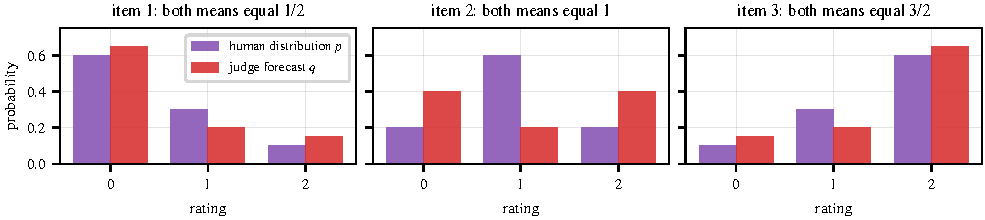
\includegraphics[width=\textwidth]{figures/fig_counterexample.pdf}
\caption{\textbf{Exact counterexample ($K=3$ ratings 0, 1, 2; $n=3$ items).}
Purple bars: the human rating distribution $P_i$; red bars: the judge's forecast $q_i$.
Both have the same item means ($\tfrac12$, $1$, $\tfrac32$), so the Pearson correlation between forecast means and human means is exactly 1.
The forecast is nevertheless wrong in shape: mean total variation distance to the human distributions $0.20$ (lower is better, range 0--1), excess RPS $3/200=0.015$ (range 0--1, lower is better), and cross-entropy $1.065$ nats against $0.915$ nats for the true distributions (CE of $P$ against itself is its entropy).
Every number is exact; no ratings are sampled.
\textbf{Takeaway:} correlation one does not imply the right distribution, and CE and RPS separate the two forecasts.}
\label{fig:counterexample}
\end{figure*}

\paragraph{An exact example.}
\Cref{fig:counterexample} gives three items on three ratings with human distributions $P_1=(0.6,0.3,0.1)$, $P_2=(0.2,0.6,0.2)$ and $P_3=(0.1,0.3,0.6)$.
The forecast matches every item mean, so $\rho=1$, yet its rating variances are $11/20$, $4/5$ and $11/20$ against $9/20$, $2/5$ and $9/20$ for the humans (derivation and table in \appref{app:proofs}; a committed script reproduces it in \expref{27}).

\paragraph{What this does not say.}
The propositions concern the set of population optima.
They do not say that every correlation-trained judge lands on a wrong shape; initialization, regularization, tie rules and model restrictions can select the true distribution from the optimum set, and a nonlinear judge may recover it from features.
They also give no universal break-even sample size.
The heuristic $N\approx P/(2B)$, from the regular asymptotic excess CE $P/(2N)$ of a $P$-parameter maximum-likelihood fit against a fixed excess CE $B$ of the competitor, holds only in CE nats under its asymptotic assumptions and cannot take an RPS gap in place of $B$.
How many ratings a cross-entropy fit needs is therefore an empirical question, and the rest of the memo measures it.

\section{Controlled studies with known rating distributions}
\label{sec:controlled}

% Provenance: experiments 01, 04, 05, 06, 07, 08, 11, 13 (archived), 15, 17, 18, 20. Every number below is printed by the script in that folder.
Synthetic items have a known $p(r\mid x)$, so every forecast can be scored exactly against the truth.
These studies cannot show that the findings transfer to human ratings; they show which mechanisms exist, and their sign and size, before any real data enter.
All of them train two judges that are identical except for the objective and score them on fresh items with RPS excess (the RPS of the forecast minus the RPS of the true distribution; zero is the best possible).

\paragraph{Proper losses separate what means cannot (experiments 01, 04, 05).}
Among nine fixed candidate forecasts, CE picked the true distribution in 249 of 256 draws with one sampled rating per validation item, and Brier and RPS in 245 of 256; all three picked it in 256 of 256 draws with two or three ratings.
Pearson, Spearman, Kendall and scaled squared error always tied all five same-mean candidates.
In the 11-artifact population of experiment 04 the maximum-entropy forecast with the human mean has Pearson correlation 1 and pays $0.117$ nats of excess CE per rating on average (item range $0.020$ to $0.210$), and three forecasts with correlation 1 differ by $0.117$ to $3.635$ nats of KL to the truth.
A forecast with the same mean, variance and every reliability coefficient as the truth still has mean TVD $0.446$ and excess RPS $0.0167$, and among five historical judges the most repeatable had the worst held-out RPS.
Variance-component tools remain useful for what they measure (\appref{app:extra}); our argument concerns the distribution of ratings, not those tools in their own role.

\paragraph{Training judges on known distributions (experiments 06, 07, 08, 18, 20).}
\Cref{tab:controlled} lists where the cross-entropy-trained judge starts to beat correlation-trained judges on held-out RPS excess.
With informative means, CE training wins from about a dozen ratings; when the mean says little and the spread carries the signal (scenario A of experiment 08), the Pearson-trained judge is better up to 96 ratings.
In experiment 20, CE wins from 16 items with three ratings each, by $+0.034$ RPS excess ($95\%$ interval $[0.031,0.036]$; CE better in 96\% of 200 seeds), and loses at 4 items by $-0.027$ ($[-0.032,-0.021]$; CE better in 24\% of seeds) because it overfits while the Pearson-trained judge stays near a uniform forecast: the test CE of the CE-trained judge is 6.14 nats against 1.83 nats for the Pearson-trained judge.
A rank correlation or a half-and-half mix of Pearson and Spearman does not change the picture (experiment 06), and larger optimizer budgets with best-of-five restarts find a better training objective in 57--90\% of the correlation fits but leave every held-out RPS crossover unchanged (experiment 07).
Pearson objectives are not convex and we have no global-optimum certificate, but within the budgets we tried the gap is not an optimizer artifact.

\begin{table}[t]
\caption{\textbf{Where CE-trained judges overtake correlation-trained judges on synthetic ratings with known distributions.}
Metric: held-out RPS excess, the RPS of the forecast minus the RPS of the true distribution on fresh items (0 is best; lower is better).
Rows read ``CE-trained better from'' the training size listed, with ratings counted in total (3 per task in experiments 06 and 08).
Training sizes: 4 to 2,048 tasks or items.
\textbf{Takeaway:} CE needs about a dozen ratings when the mean is informative and more than 96 when it is not.}
\label{tab:controlled}
\centering\small
\begin{tabular}{@{}p{0.34\columnwidth}p{0.58\columnwidth}@{}}
\toprule
Study & CE-trained better from \\
\midrule
Exp.\ 08, scenarios B, C, D & 12 ratings (4 tasks) \\
Exp.\ 08, scenario A (mean uninformative) & more than 96 ratings; Pearson wins to 32 tasks \\
Exp.\ 06, scenario B / A, vs.\ Spearman, Kendall, mixed & 12 ratings / 192 ratings (64 tasks) \\
Exp.\ 20, 3 ratings per item & 48 ratings (16 items); loses at 12 ratings (4 items) \\
Exp.\ 20, 1 rating per item & 32 items \\
Exp.\ 18, vs.\ Pearson-trained & 16 items (10 ratings each), 32 (3), 64 (1), median over 12 settings \\
\bottomrule
\end{tabular}
\end{table}

\paragraph{A calibrated head closes much of the gap (experiments 11, 15, 17, 18).}
Squared-error training fixes Pearson's drift in level and scale, and a calibration head after a Pearson score fixes the rest of what a scalar can fix, yet squared error leaves conditional higher moments unconstrained: at 2{,}048 items it trails the validation-selected CE fit by $0.0069$ to $0.0087$ RPS excess (all intervals above zero; experiment 11).
A flexible calibrator on the \emph{true} mean matches or beats end-to-end CE from 512 items (experiment 17), and a Pearson score followed by a calibrated affine head beats CE-trained judges from 128 items when the spread is a function of the mean but loses when the spread varies independently of it (experiment 18).
The shape has to be fitted, and CE is one way to fit it.
Rater severity does not change the picture: offsets are about $0.1$ rating points and leave the RPS ranking unchanged (Kendall $\tau\ge0.995$; experiment 15).
Details of these studies are in \appref{app:extra}.

\section{Frozen frontier judges on human ratings}
\label{sec:frozen}

% Provenance: experiments 21, 23, 26, 28 (frozen judges, calibration head); 02, 09, 10, 12, 14, 16, 18, 19, 20 (75 retrospective VeriBench artifacts).
Here the foundation model stays frozen and we calibrate only its reported category probabilities, so the comparison isolates the training objective from judge quality.
Each judge forecast $p$ passes through the 27-setting head of Equation~\eqref{eq:head}.
A CE fit and a Pearson fit choose among the same settings from the same training ratings (\appref{app:protocols}).
Experiment 28 has the widest coverage: five frontier judges (GPT-6 Astra, Claude Opus 5.5, Kimi K3, GLM 5.3, DeepSeek V4.1 Flash) on 2{,}350 label-free requests from five public rating sets.
Three come from ChaosNLI~\citep{nie2020chaosnli}, with 100 human labels per item: random subsets of the SNLI (600 items), MNLI-matched (600) and alphaNLI (400) parts.
Two are the chatbot-safety sets of DICES~\citep{aroyo2023dices}: DICES-350 (all 350 conversations, 123 ratings each) and DICES-990 (400 conversations, 69--76 ratings each).
We fixed the protocol and the request hashes before any judge call or label join.
Pearson and RPS inherit an ordinal coding that is an assumption: we read entailment as agreement and DICES as a harm scale (No $<$ Unsure $<$ Yes).
The SNLI and MNLI-matched parts keep only items whose original labels were not unanimous, so they over-represent disagreement.
AlphaNLI has two classes, so its mean fixes the distribution, and it serves as a control.
We test on held-out folds and score each held-out item against its entire empirical human distribution, with 200 training draws per fold and condition.
Budgets run from 4 to 256 ratings with one rating per item and from 10 to 320 ratings with five per item.

\begin{figure*}[t]
\centering
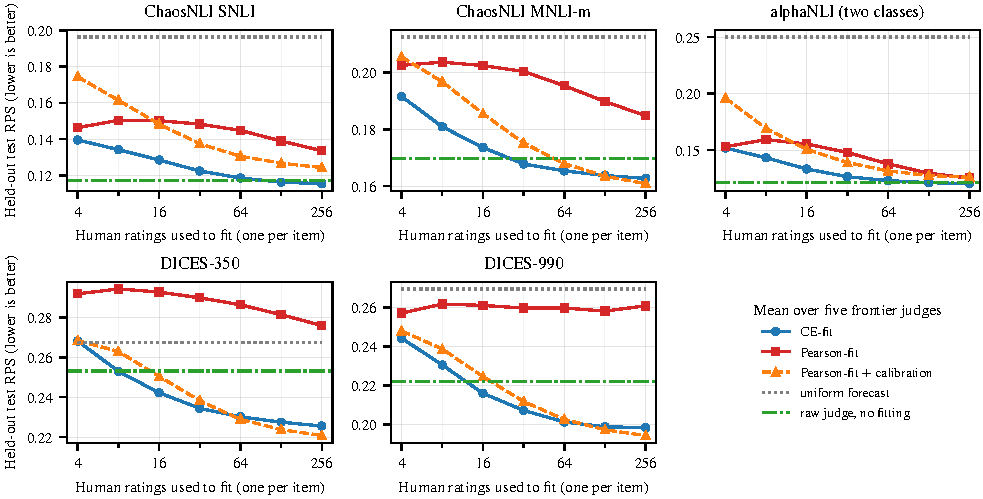
\includegraphics[width=\textwidth]{figures/fig_exp28.pdf}
\caption{\textbf{CE-fit passes the uniform forecast and Pearson-fit after a handful of ratings, but the unfitted judge is hard to beat on ChaosNLI, and a calibrated Pearson fit ends slightly lower on MNLI-matched and DICES.}
Learning curves of frozen judges with a calibration head on five public rating sets.
Vertical axis: held-out test ranked probability score (RPS), mean over the five frontier judges (0--1; lower is better); horizontal axis: number of human ratings spent on fitting, one rating per item.
Test data: held-out folds of ChaosNLI (SNLI, MNLI-matched, alphaNLI) and DICES (DICES-350 with 350 conversations, DICES-990 with a 400-conversation sample), each item scored against its full empirical human distribution; 200 training draws per fold.
Blue: CE-fit; red: Pearson-fit; orange dashed: Pearson-fit followed by distribution calibration on the same ratings; dotted gray: uniform forecast; dash-dotted green: the judge's raw forecast with no fitting.
Both fits search the same 27 calibration settings exhaustively (ties to the setting nearest the identity), so each is the exact optimum within that family.
No interval is drawn (see \Cref{tab:exp28}).}
\label{fig:exp28}
\end{figure*}

\paragraph{Result.}
CE-fit beats Pearson-fit and a uniform forecast on held-out RPS after 4 to 8 ratings with one rating per item, or after 10 to 20 ratings with five per item, in all 25 judge-by-dataset cells.
The simultaneous one-sided 97.5\% lower bounds of both differences stay above zero from the listed break-even budget $N^\ast$ to the largest tested (\Cref{tab:exp28}).
At the largest budget CE-fit has the lower mean RPS in all 50 judge-by-dataset-by-condition cells.
Across all 325 comparison cells, Pearson-fit has the lower mean RPS in 25 (three at four ratings with one per item and 22 at ten ratings with five per item, where four or two training items give a correlation very little to work with), significantly so in 19.
On DICES, where the Pearson-fit curve is flat, the gap is large: at 256 ratings the mean RPS is 0.226 for CE-fit against 0.276 for Pearson-fit on DICES-350 and 0.198 against 0.261 on DICES-990.

\begin{table*}[t]
\caption{\textbf{A handful of ratings suffices to beat both baselines, but at 256 ratings the calibrated Pearson fit equals or beats the cross-entropy (CE) fit on MNLI-matched and on both DICES sets.}
Held-out ranked probability score (RPS) at 256 human ratings (one per item) and break-even budgets, experiment 28.
Mean over five frontier judges; RPS in $[0,1]$, lower is better; bold marks the lowest value in the row.
Unif.: uniform forecast; Raw: the judge's own forecast with no fitting; Pearson-fit+cal.: a Pearson fit followed by train-only calibration of grade frequencies in four quantile bins of the expected score.
$N^\ast$: the smallest number of training ratings from which the simultaneous one-sided 97.5\% lower bounds of ``test RPS of the Pearson-fit judge minus test RPS of the CE-fit judge'' and ``test RPS of the uniform forecast minus test RPS of the CE-fit judge'' both stay above zero at every larger budget; ranges are across the five judges, with one (1/item) and five (5/item) ratings per item.
Test: held-out folds of each rating set, 200 training draws per fold; 4{,}000 bootstrap resamples of held-out items; both fits search the same 27 calibration settings exhaustively.}
\label{tab:exp28}
\centering\small
\begin{tabular}{lrrrrrcc}
\toprule
Rating set & Unif. & Raw & CE-fit & Pearson-fit & Pearson-fit+cal. & $N^\ast$ (1/item) & $N^\ast$ (5/item) \\
\midrule
ChaosNLI SNLI & 0.196 & 0.117 & \textbf{0.115} & 0.134 & 0.124 & 4 & 20 \\
ChaosNLI MNLI-m & 0.213 & 0.170 & \textbf{0.163} & 0.185 & 0.161 & 4 & 20 \\
alphaNLI (two classes) & 0.250 & 0.121 & \textbf{0.120} & 0.125 & 0.126 & 4--8 & 20 \\
DICES-350 & 0.267 & 0.253 & \textbf{0.226} & 0.276 & 0.221 & 8 & 10--20 \\
DICES-990 & 0.269 & 0.222 & \textbf{0.198} & 0.261 & 0.194 & 4 & 20 \\
\bottomrule
\end{tabular}

\end{table*}

\paragraph{CE is one way to fit the shape, not the only way.}
Against the unfitted judge the fitted head often loses: the raw forecast has significantly lower RPS than CE-fit in 156 of 325 cells (134 on ChaosNLI, where strong frontier judges already forecast the distribution well) and in 17 of 25 at eight ratings with one per item.
CE-fit has a sustained win over it (lower bound above zero at every larger budget) in 28 of 50 judge-by-set-by-condition cells: 2 of 10 on SNLI and on alphaNLI, 6 of 10 on MNLI-matched, 10 of 10 on DICES-350 and 8 of 10 on DICES-990.
A Pearson fit followed by calibration into grade frequencies, itself a proper-loss step, has lower mean RPS than CE-fit with one rating per item from 64 ratings on DICES-350 and from 128 on DICES-990 and MNLI-matched, by a few thousandths at 256 ratings (\Cref{tab:exp28}).
We read this as support for the argument, not a counterexample: what fails is selection or training by correlation \emph{alone}, and any step that fits the shape with a proper loss repairs it.

\paragraph{Other human ratings agree in direction and are mixed in size.}
\appref{app:extra} gives details and tables.
(1) On 160 student homework answers graded twice, CE-fit has lower held-out RPS than Pearson-fit for each of five frontier judges at every one of seven budgets (35 of 35 cells).
The preregistered descending test passes down to 8 ratings for two judges and fails at 256 for three (experiments 21 and 26).
For Qwen3.5-9B at 256 ratings the Pearson fit has the higher held-out correlation ($0.620$ against $0.556$) yet predicts a mean grade of $2.79$ for a human mean of $4.31$.
(2) On public benchmarks with a weaker judge (KonIQ-10k, SummEval, dialogue, MovieLens; experiment 23), direct CE selection beat direct Pearson selection at the largest budget on three of the four; on SummEval the Pearson fit won (RPS $0.144$ against $0.284$ at 768 ratings, the CE fit having selected the uniform forecast).
The margin over strong controls is small or absent in all four, and a calibrated Pearson score did at least as well as CE at the largest budget in all four.
(3) On the 75 retrospective theorem artifacts (195 expert ratings; Section~\ref{sec:limits} lists the experiments that reuse them), CE-trained mixtures and heads have lower test RPS than Pearson-trained ones in most pools and sizes, by $0.003$ to $0.090$ (experiments 10, 18 and 20).
At three training families CE ties on three pools and loses on the open-weight pool (experiment 20).
Choosing a single judge depends on the pool.
Selection by Pearson matched or beat selection by CE on the 44 historical scalar-vote judges, whereas selection by CE won on the 15 closed-weight judges with native probabilities, the 39 open-weight judges with three scalar votes and the combined 59 (experiment 20).
Pool format and model weights are confounded.

\section{Trained judges: matched LoRA fine-tuning with four objectives}
\label{sec:lora}

% Provenance: experiments 24, 25 (HelpSteer2) and 29 (ChaosNLI, DICES, HelpSteer2; 1,401 of 1,401 runs verified).
Calibrating a frozen judge changes only its output map.
To test whether the objective also changes what the judge learns, experiments 24, 25 and 29 fine-tune the weights.
We adapt Qwen3-4B-Instruct-2507 and Llama-3.1-8B-Instruct with LoRA~\citep{hu2022lora} (rank 8, $\alpha=16$, top four transformer blocks, plus a rating read-out) on human ratings of HelpSteer2 helpfulness~\citep{wang2024helpsteer2} (five ordinal levels, 1{,}038 held-out responses from 519 held-out prompts), ChaosNLI, DICES and the two-class alphaNLI.
We train four objectives: CE, RPS, mean squared error on the expected rating, and Pearson correlation.
Model, prompt, optimizer (AdamW), three learning rates, mini-batch schedule and validation-RPS selection among four checkpoints are identical across them.
A raw forecast is the network's output.
A calibrated forecast adds a one-dimensional score calibration (1D) or a $(K+2)$-parameter logit calibration fitted on separate ratings, identically for every objective.
Intervals are simultaneous maximum-$t$ 95\% cluster-bootstrap bands over held-out clusters with 4{,}000 draws, both conditional on the matched training draws and crossed with them (draw by held-out unit).

\begin{figure*}[t]
\centering
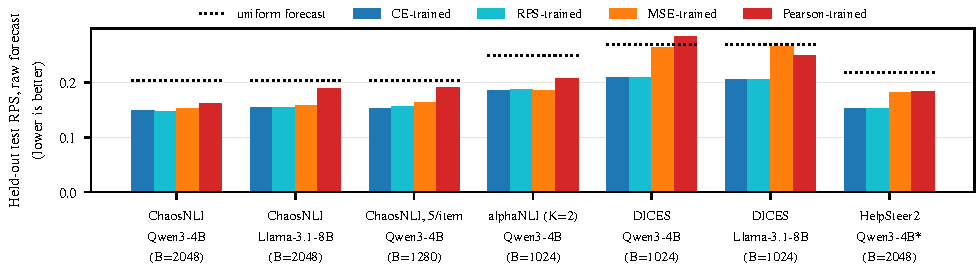
\includegraphics[width=\textwidth]{figures/fig_exp29_four_objectives.pdf}
\caption{\textbf{Pearson-trained judges have higher raw ranked probability score (RPS) than CE-trained judges in all seven setups at the largest budget.}
Four training objectives for LoRA judges at the largest budget, raw forecast.
Vertical axis: held-out test RPS of the network's own forecast, with no post-hoc calibration (0--1; lower is better); the dotted line is the uniform forecast.
Blue: CE-trained; cyan: RPS-trained; orange: MSE-trained; red: Pearson-trained.
Horizontal axis: dataset, base model and development budget $B$ in ratings (one per item unless ``5/item''); half of $B$ trains the weights, and a quarter each selects the checkpoint and fits the calibration.
Test data: held-out items or prompts of ChaosNLI, DICES and HelpSteer2 ($K=2$ for alphaNLI, 3 for ChaosNLI and DICES, 5 for HelpSteer2).
Each judge is the checkpoint with the lowest validation RPS among three learning rates and four checkpoints; no objective is given more search.
*\,HelpSteer2 CE and Pearson bars reuse experiment 24 predictions; RPS and MSE bars are new. Part of each test set was scored in experiment 28 (Section~\ref{sec:limits}).
No interval is drawn (crossed bands: \Cref{tab:exp29}).}
\label{fig:exp29}
\end{figure*}

\paragraph{Result.}
At the largest budget in every one of the seven setups, the Pearson-trained judge has the higher held-out RPS.
The test RPS of the Pearson-trained judge minus the test RPS of the CE-trained judge is positive in every setup, with a crossed simultaneous 95\% band above zero: $+0.0132$ to $+0.0761$ (\Cref{fig:exp29}; per-setup values in \appref{app:extra}).
The RPS-trained judge is within $0.003$ of the CE-trained judge in absolute test RPS in every setup, as expected for two strictly proper scores; against the Pearson-trained judge, sustained crossed wins begin at 16 to 80 ratings for CE and at 64 to 1{,}024 for RPS, depending on the setup.
Mean squared error is the instructive case.
At $K=2$ (alphaNLI) the mean fixes the distribution, and the squared-error judge is close to CE: the test RPS of the squared-error judge minus that of the CE judge is $+0.0003$ (interval $[-0.0021,+0.0028]$ includes zero; no equivalence margin set).
At $K\ge3$ the CE-trained judge beats the squared-error judge on five of six panels at the crossed 95\% level, by $0.003$ to $0.061$ RPS.
The exception is Llama-3.1-8B on ChaosNLI ($+0.0025$ with crossed interval $[-0.0007,+0.0057]$).
The squared-error judge beats the Pearson-trained judge on three of six.
Shape information that squared error leaves unidentified is worth the most where disagreement is largest: on DICES, the squared-error judge scores $0.264$ and $0.267$ against $0.209$ and $0.206$ for CE.

\paragraph{After calibration the gap nearly closes.}
With one shared post-hoc one-dimensional calibration the difference between the two objectives shrinks to $0.0002$ to $0.0043$ test RPS across the seven setups of experiment 29 ($0.0004$ to $0.0033$ with the logit calibration), and the CE-trained judge stays ahead in point estimate in all seven.
A sustained advantage then appears under the conditional simultaneous band in four setups for the one-dimensional calibration and in five for the logit calibration, never on DICES.
Under the stricter crossed band it appears in two setups for each calibration.
On alphaNLI, a binary target where the mean fixes the distribution, the one-dimensional difference is $+0.0043$ (crossed interval $[+0.0006,+0.0080]$, CE ahead in 10 of 10 draws), so a residual gap remains.
The larger HelpSteer2 studies agree (experiments 24 and 25; \Cref{fig:lora-hs2} in \appref{app:extra}).
At 2{,}048 ratings the calibrated difference is $+0.0011$ on Qwen3-4B (conditional 95\% interval $[+0.0002,+0.0020]$, crossed $[-0.0003,+0.0025]$) and $-0.0011$ on Llama-3.1-8B (conditional interval $[-0.0023,+0.0001]$; negative favors the Pearson-trained judge); on Qwen3-4B it is $+0.0001$ at 8{,}192 ratings, with no sustained win.

Taken together, the training objective matters most for the raw forecast, where a correlation objective is weakest: Pearson is blind to level and scale, so the mean of a Pearson-trained judge is off by an arbitrary affine map.
In experiment 24 the raw Pearson LoRA has RPS $0.18376$ against $0.15213$ for CE at 2{,}048 ratings, with a mean bias (forecast mean minus human mean) of $+0.126$ against $-0.035$.
An identical proper-loss calibration repairs most of that, and the remaining gap is small and model-dependent, as in the controlled studies of Section~\ref{sec:controlled}: once level and scale are fixed, what remains is the quality of the learned score.

\section{Scaling laws for judges}
\label{sec:scaling}

% Provenance: experiment 31 (free CPU re-analysis of the saved results of experiments 26, 28 and 29; no model calls).
If a judge is an ordinary learning problem, its held-out loss should fall with data the way other losses do.
We fit a saturating power law to the saved learning curves of experiments 26, 28 and 29,
\begin{equation}
\mathrm{error}(N)=\mathrm{floor}+a\,(N/N_{\min})^{-b},
\label{eq:scaling}
\end{equation}
where $N$ is the number of human ratings spent on fitting, $a$ is the excess at the smallest $N$ tested, $b\in[0.02,3]$ and $\mathrm{floor},a\ge0$.
The scaling-law literature~\citep{kaplan2020scaling,hoffmann2022training} treats cross-entropy as the quantity that falls smoothly with data, so we ask whether the curves of a CE-fit judge follow Equation~\eqref{eq:scaling} and whether those of a Pearson-fit judge do.
We fit by weighted least squares with weights $1/\mathrm{SE}^2$ from the saved standard errors, exactly over a grid of 150 values of $b$, and take percentile 95\% intervals from 2{,}000 parametric bootstrap draws per curve.
A curve is non-monotone if any step up exceeds 1.96 standard errors, flat if it declines by under two standard errors, and poorly fit if the root-mean-square residual exceeds 10\% of its range; its floor is not identified if the floor's interval is wider than that range.
We do not fit curves with three budgets.

\begin{figure*}[t]
\centering
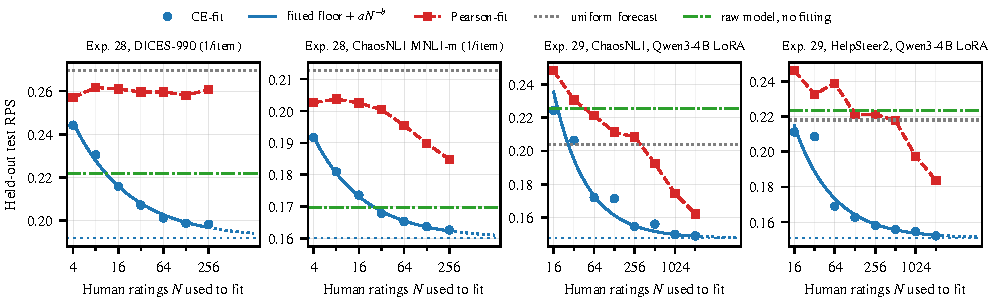
\includegraphics[width=\textwidth]{figures/fig_scaling.pdf}
\caption{\textbf{CE curves saturate with the number of human ratings in most panels; Pearson curves are flat or still falling at the largest budget.}
Held-out ranked probability score (RPS) against the number of human ratings, with a saturating power-law fit for the CE-fit judge.
Vertical axis: held-out test RPS (0--1; lower is better); horizontal axis: number of human ratings $N$ used to fit (log scale).
Left two panels: frozen frontier judges with a 27-setting head, mean over five judges, one rating per item, on DICES-990 and ChaosNLI MNLI-matched (experiment 28).
Right two panels: raw (uncalibrated) forecasts of CE-trained and Pearson-trained LoRA judges, Qwen3-4B-Instruct on ChaosNLI and HelpSteer2 (experiment 29; 10 draws per budget).
Blue: CE-fit or CE-trained, with the fitted $\mathrm{floor}+aN^{-b}$ (solid over the tested range, dotted beyond it); red dashed: Pearson-fit or Pearson-trained; dotted: uniform; dash-dotted green: the untuned model.
The CE judge is chosen by minimizing training cross-entropy within its family (exhaustive search for the head; AdamW with a validation-selected checkpoint for LoRA); the Pearson judge is chosen the same way with correlation as objective.
No interval is drawn (fits with intervals: \Cref{tab:scaling}).}
\label{fig:scaling}
\end{figure*}

\paragraph{CE curves usually follow a saturating power law.}
Equation~\eqref{eq:scaling} fits the CE curve in 9 of the 11 panels; \Cref{tab:scaling} in \appref{app:extra} lists every panel, its fit verdict and its floor.
For the frozen judges of experiment 28 with one rating per item, it fits all 25 judge-by-dataset cells on RPS but identifies the floor in only 8.
Where the floor is identified, the median exponent is $0.66$ for RPS (8 of 25 cells), $0.82$ for cross-entropy (20 of 25) and $0.59$ for total variation distance (10 of 25).
For CE-trained LoRA on the three experiment 29 panels with eight budgets, $b$ is $0.89$ (95\% interval $[0.76,0.99]$) on ChaosNLI with Qwen3-4B, where the law fits; the other two panels have $b$ of $0.76$ and $0.64$ but residuals above the 10\% rule (\Cref{tab:scaling}).

\paragraph{Pearson curves rarely do.}
Equation~\eqref{eq:scaling} fits the Pearson curve in one of the eleven panels, ChaosNLI with Qwen3-4B, with $b=0.09$ and an extrapolated floor of $0.002$, which is implausible when raters disagree.
Eight Pearson curves fit poorly and two are flat (DICES-990 stays at RPS $0.26$ against $0.27$ for uniform).
All 25 judge-by-dataset cells with five ratings per item are non-monotone.
At the largest $N$ tested, the Pearson-fit RPS lies above the CE-fit floor in 20 of 25 experiment 28 cells with one rating per item at a 95\% bound (cross-entropy: 25 of 25; TVD: 21 of 25), so the Pearson curve has not reached where the CE curve saturates and the data cannot say whether it does.
The result concerns these two objectives in these families, not every correlation objective with every optimizer.

\paragraph{What we cannot say.}
The fits are indications, not laws.
The saved standard errors are approximate, and those of experiment 26 are too wide to identify any law; we estimate no human leave-one-vote-out floor; nothing is observed beyond 320 ratings (experiments 26 and 28) or $2{,}048$ (experiment 29), so the dotted extrapolations in \Cref{fig:scaling} are extrapolations; and the exponents describe five rating sets, two model families and two training methods.
\appref{app:extra-tables} lists every caveat.

\section{Limitations, negative results and recommendations}
\label{sec:limits}

\paragraph{Where correlation holds up.}
Five results argue against a blanket preference for CE.
(1) With very few ratings the Pearson-fit judge sometimes wins.
In experiment 28 it has the lower mean RPS in 25 of 325 cells, significantly so in 19, all at the smallest budgets (Section~\ref{sec:frozen}), and in the synthetic studies a CE-trained judge overfits at 4 items (Section~\ref{sec:controlled}).
(2) When the mean says little and the spread carries the signal, the order reverses in the synthetic studies (scenario A), up to 96 ratings.
(3) Selecting a single judge by Pearson matched or beat selecting it by CE among the 44 historical scalar-vote theorem judges, though not in the other three pools (Section~\ref{sec:frozen}; experiment 20).
(4) A Pearson score followed by a proper-loss calibration into grade probabilities equals or beats the CE fit on DICES, KonIQ, SummEval, dialogue and MovieLens, and after one shared calibration the LoRA gap shrinks to $0.0002$ to $0.0043$ RPS.
(5) Three of the five frontier judges on the homework answers do not clear the preregistered descending test at 256 ratings, and Claude Sonnet 5 never passes it.
Where a distribution is needed, correlation alone was the weaker training signal in most of our comparisons; the gain comes from fitting the distribution with a proper loss, by whichever route.

\paragraph{What the evidence does not show.}
The evidence is partly retrospective and partly shared.
Experiments 02, 09, 10, 12, 14, 16, 18, 19 and 20 reuse the same 75 theorem artifacts and 195 expert ratings, so together they form one body of evidence.
Experiment 29's HelpSteer2 CE and Pearson curves reuse experiment 24's predictions, and its test items overlap experiment 28's frontier-scored items (265 of 713 ChaosNLI, 110 of 412 alphaNLI and 172 of 300 DICES items), although the LoRA judges never trained on them.
We do not know whether a pretrained model saw a public benchmark.
The bands condition on the training draws and, for experiment 28, on the item subsample; ten homework assignments in one course with two graders are ten dependent folds.
Pearson and RPS both inherit the ordinal coding of the NLI and DICES categories, which is an assumption, and SNLI and MNLI-matched keep only items with non-unanimous original labels.
We collected no new human ratings for this memo, and the intended application, a theorem-judge rating collection owned by the sister repository, has no fresh ratings yet.
We estimate no human leave-one-vote-out floor for the fitted curves (Section~\ref{sec:scaling}).
For trained judges (the toy models and LoRA), Pearson objectives are not convex and we have no global-optimum certificate: the restarts of experiment 07 change no crossover but cannot prove that none exists, whereas the exhaustive head search of experiments 21, 26 and 28 and the mixture fits of experiment 02 are exact within their families.
The identification propositions concern population optimum sets, not the learning dynamics of any one optimizer.

\paragraph{Recommendations.}
\begin{enumerate}
\item \textbf{Fit judges on individual ratings with a proper loss} (CE, or RPS for ordinal scales) and report held-out RPS, CE and TVD, with correlations as secondary ranking diagnostics.
\item \textbf{Keep the baselines in every table:} the uniform forecast, the training histogram and the unfitted judge.
\item \textbf{Calibrate the distribution even when you select by ranking.} A ranking-selected score with a calibrated head is a strong, cheap comparator.
\item \textbf{Report learning curves with simultaneous intervals} and name the data, the metric and the direction of every difference; do not report one correlation.
\item \textbf{Budget about eight ratings with one rating per item, or twenty with five per item, to fit a calibration head to a strong frozen judge} (the largest break-even budgets over the 25 cells of experiment 28), then \textbf{treat the training objective as a second-order choice once the output is calibrated}: after one shared calibration the CE-trained and Pearson-trained LoRA judges differ by $0.0002$ to $0.0043$ RPS (Section~\ref{sec:lora}).
\end{enumerate}
The common thread follows the blog post~\citep{miranda2026bitter}: judges pose an ordinary supervised learning problem, so loss choice, held-out data and learning curves apply as they do to any other model.


\section*{Acknowledgments}
We thank Sanmi Koyejo for repeated technical feedback that shaped experiments 11, 15--17 and 22.

\bibliography{memo_refs}
\bibliographystyle{icml2026}

\newpage
\appendix
\onecolumn
\section{Proofs and derivations}
\label{app:proofs}

Notation follows Section~\ref{sec:identification}: $P_i$ and $q_i$ are distributions on $\{0,\dots,K-1\}$ with means $t_i$ and $m_i$, $F_q(k)=\sum_{r\le k}q(r)$ for $k=0,\dots,K-2$, and $d_k=F_P(k)-F_q(k)$.
Logarithms are natural; entropy $H$, cross-entropy $\CE$ and $\KL$ are in nats.
The statements are those of the identification preprint~\citep{miranda2026correlation}; we repeat the proofs so that the memo is self-contained.

\subsection{Pearson depends on means up to a positive affine map (Proposition~\ref{prop:affine})}
Since $\sum_i(t_i-\bar t)=0$, $\sum_i(m_i-\bar m)(t_i-\bar t)=\sum_i m_i(t_i-\bar t)=\sum_i(t_i-\bar t)\sum_r r\,q_i(r)$.
The numerator is linear in the probabilities and the denominator depends on the forecast only through $m$, so forecasts with equal item means have equal correlation.
The centered vector of $a\mathbf 1+bm$ is $b(m-\bar m\mathbf 1)$; numerator and standard deviation of the forecast both acquire the factor $b>0$, so $\rho$ is unchanged.
Cauchy--Schwarz bounds $\rho$ by one, with positive equality exactly when $m-\bar m\mathbf 1=b(t-\bar t\mathbf 1)$ for some $b>0$; setting $a=\bar m-b\bar t$ gives $m=a\mathbf 1+bt$.
The map $x\mapsto m(x)$ is unrestricted: the statement is about the output vector of means.

\subsection{Dimension of the unidentified set (Proposition~\ref{prop:dimension})}
For $K=2$, $q(1)=m$ and $q(0)=1-m$.
For general $K$ the constraints $\sum_rq(r)=1$ and $\sum_rr\,q(r)=m$ have linearly independent coefficient vectors, so their common affine solution set has dimension $K-2$; every interior mean $m\in(0,K-1)$ has an all-positive solution (the exponential family of \Cref{app:ce-gap}), so positivity adds no local equality constraint.
For $n$ items with prescribed interior means the dimensions add to $n(K-2)$.
In $m=a\mathbf 1+bt$ the columns $\mathbf 1$ and $t$ are independent because $t$ is nonconstant, which adds the two free parameters $(a,b)$ on the all-positive stratum, giving $n(K-2)+2$.
For binary ratings and correlation-one means $m_i=a+bt_i$, the Brier convention gives excess RPS $n^{-1}\sum_i(a+(b-1)t_i)^2$ and excess CE $n^{-1}\sum_i\KL(\mathrm{Bern}(t_i)\|\mathrm{Bern}(a+bt_i))$, so binary ratings keep level and scale ambiguity (the squared-error-over-both-categories convention would double the first expression).
For $K=3$ and mean one, the family $q_s=(s,1-2s,s)$, $0\le s\le\tfrac12$, has variance $2s$ at fixed mean.

\subsection{What each objective identifies (Proposition~\ref{prop:losses})}
\emph{Squared error.} For any $a$, $\E[(a-R)^2\mid x]=(a-\E[R\mid x])^2+\Var(R\mid x)$; the minimizer over $a$ is the conditional mean and the second term does not depend on $a$.

\emph{Cross-entropy.} $\CE(P,q)=H(P)+\KL(P\|q)$.
With $A=\{r:P(r)>0\}$ and $q$ positive on $A$, concavity of the logarithm gives $-\KL(P\|q)=\sum_{r\in A}P(r)\log(q(r)/P(r))\le\log\sum_{r\in A}q(r)\le0$, with equality only if $q/P$ is constant on $A$ and $q(A)=1$, that is $q=P$.
If $q$ vanishes on a category of positive $P$-mass, $\CE=+\infty$.

\emph{RPS.} Let $Z_k=\mathbf 1\{Y\le k\}$ with $Y\sim P$, so $\E Z_k=F_P(k)$ and $\Var Z_k=F_P(k)(1-F_P(k))$.
Because $\E(a-Z_k)^2=(a-F_P(k))^2+\Var Z_k$, summing over $k$ and dividing by $K-1$ gives
\[
\E_P\RPS(q,Y)=\frac1{K-1}\sum_kF_P(k)(1-F_P(k))+\frac{D(P,q)}{K-1},\qquad D=\sum_kd_k^2 .
\]
The first term does not depend on $q$, so the excess is $D/(K-1)$.
Since $\sum_{k=0}^{K-2}F_P(k)=\sum_rP(r)(K-1-r)=K-1-m_P$, we have $\sum_kd_k=m_q-m_P$.
The centered sum-of-squares identity $\sum_kd_k^2=(\sum_kd_k)^2/(K-1)+\sum_k(d_k-\bar d)^2$ then gives Equation~\eqref{eq:rps-decomp}.
The excess is zero exactly when all CDF values agree, which fixes every category probability by successive differences, so the normalized RPS is strictly proper on the whole simplex including its boundary.
Finally, by mass conservation $m_q-m_P=\sum_r(r-\tfrac{K-1}2)(q(r)-P(r))$ and so $|m_q-m_P|\le\tfrac{K-1}2\sum_r|q(r)-P(r)|=(K-1)\TVD(P,q)$.

\emph{TVD is not a proper score for individual ratings.}
For a point mass $\delta_y$, $\TVD(q,\delta_y)=1-q(y)$, so $\E_{Y\sim P}\TVD(q,\delta_Y)=1-\sum_rP(r)q(r)$, which is minimized by forecasts supported on the modal categories of $P$ and generally does not recover $P$.
TVD to a sparse empirical histogram is a noisy diagnostic whose expectation need not equal TVD to $P$.

\subsection{CE controls bounded moments (Proposition~\ref{prop:moments})}
Let $f:\{0,\dots,K-1\}\to[0,1]$, $\delta=P-q$ and $A=\{r:\delta(r)\ge0\}$.
Since $\sum_r\delta(r)=0$, $\sum_{r\in A}\delta(r)=\TVD(P,q)=d$, and $|\sum_rf(r)\delta(r)|\le d$.
For the second inequality assume $\KL(P\|q)<\infty$; grouping categories into $A$ and its complement cannot increase KL, by concavity of the logarithm.
With $a=P(A)$ and $b=q(A)$, so $a-b=d$, the grouped bound is the Bernoulli KL $h_b(a)$, with $h_b(b)=h_b'(b)=0$ and $h_b''(a)=1/(a(1-a))\ge4$; integrating twice gives $h_b(a)\ge2(a-b)^2$, so $\KL(P\|q)\ge2\TVD(P,q)^2$ (Pinsker).
Taking $f(r)=(r/(K-1))^j$, $|m_j(q,x)-m_j(p,x)|\le\TVD(p(\cdot|x),q(\cdot|x))\le\sqrt{\KL(p(\cdot|x)\|q(\cdot|x))/2}$, and averaging the square over $X$ with $\E_X\KL(p(\cdot|X)\|q(\cdot|X))=\CE(q)-\CE(p)$ gives the claim.

\subsection{Means alone cannot recover shape (Proposition~\ref{prop:lower})}
A rule that sees only the mean must output the same $q$ under $P_0$ and $P_1$.
The triangle inequality gives $d\le\TVD(P_0,q)+\TVD(q,P_1)$, so $\max_j\TVD(P_j,q)\ge d/2$.
Let $v_j=(F_{P_j}(k))_k$ and $u=(F_q(k))_k$.
The Euclidean identity $\tfrac12(\|v_0-u\|^2+\|v_1-u\|^2)=\|u-\tfrac12(v_0+v_1)\|^2+\tfrac14\|v_0-v_1\|^2$ and the RPS identity of the previous section give $\tfrac12(\mathcal E_{P_0}(q)+\mathcal E_{P_1}(q))\ge D(P_0,P_1)/(4(K-1))$.
For the $j$ attaining the maximum TVD, Pinsker gives $\KL(P_j\|q)\ge2(d/2)^2=d^2/2$.
The mixture $\tfrac12(P_0+P_1)$ attains the total variation bound and the average excess RPS bound when it is a feasible forecast.
These are information bounds for a rule that receives only the mean; they do not bound an estimator that also sees individual ratings, features or shape restrictions.

\subsection{Gradients}
Let $q_i=\mathrm{softmax}(u_i)$, $\zeta_i=(t_i-\bar t)/s_t$, $z_i=(m_i-\bar m)/s_m$, $T=t-\bar t\mathbf 1$, $C=m-\bar m\mathbf 1$ and $N=T^\top m$, so $\rho=N/(\|T\|\|C\|)$.
Then $\partial N/\partial m_i=T_i$ and $\partial\|C\|/\partial m_i=C_i/\|C\|$ because $\sum_iC_i=0$, and the quotient rule gives $\partial\rho/\partial m_i=g_i=(\zeta_i-\rho z_i)/(ns_m)$.
The softmax derivative $\partial q_i(s)/\partial u_i(r)=q_i(s)(\mathbf 1\{s=r\}-q_i(r))$ gives $\partial m_i/\partial u_i(r)=q_i(r)(r-m_i)$, hence $\partial\rho/\partial u_i(r)=g_iq_i(r)(r-m_i)$.
Differentiating $-\sum_sP_i(s)\log q_i(s)$ gives $q_i(r)-P_i(r)$.
For a differentiable shared-parameter model, $D\rho(\theta)[v]=\sum_ig_iDM_i(\theta)[v]$ vanishes whenever $DM(\theta)[v]=0$; this is a first-order statement at a point and not a statement about higher-order changes.

\subsection{The exponential family, the signed CE decomposition and the entropy gap}
\label{app:ce-gap}
Let $q_\gamma(r)=e^{\gamma r-A(\gamma)}$ on $\{0,\dots,K-1\}$ with $A(\gamma)=\log\sum_re^{\gamma r}$.
Then $A'(\gamma)=m(\gamma)$ and $A''(\gamma)=\Var_{q_\gamma}(R)>0$, so the mean map is a strictly increasing bijection from $\mathbb R$ onto $(0,K-1)$.
For a target $P$ with interior mean $t$, $\CE(P,q_\gamma)=-\gamma t+A(\gamma)$ is strictly convex in $\gamma$ with derivative $m(\gamma)-t$, so its unique minimizer is the mean-matching member $q_t$.
For any $P$ with mean $t$, $\KL(P\|q_t)=-H(P)-\gamma t+A(\gamma)=H(q_t)-H(P)$, so $q_t$ is the unique maximum-entropy distribution with mean $t$.
Define the gap $G(P)=H(q_t)-H(P)\ge0$: it is the excess CE of the best forecast that is log-affine in the rating.
For any $q$ positive on every category, adding and subtracting $\CE(q_t,q)=H(q_t)+\KL(q_t\|q)$ gives
\[
\CE(P,q)=H(P)+G(P)+\KL(q_t\|q)+C(P,q),\qquad C(P,q)=\sum_r(P(r)-q_t(r))(-\log q(r)).
\]
The cross term vanishes when $\log q(r)=\alpha+\beta r$, because $P$ and $q_t$ share total mass and mean, and it can be negative: at $q=P$, $C(P,P)=-G(P)-\KL(q_t\|P)$.
The gap is therefore a restriction cost for the log-affine family and not an unavoidable penalty on every forecast.
In the 11-artifact population of experiment 04 ($p_x=0.9\,\mathrm{Binomial}(5,j/12)+0.1\,\mathrm{Uniform}$), the mean gap is $0.117$ nats (item range $0.020$ to $0.210$), against the largest possible entropy $\log6=1.792$ nats.
Locally, $\KL(q_{\gamma_t}\|q_{\gamma_m})=(m-t)^2/(2A''(\gamma_t))+o((m-t)^2)$, the cost of a mean miscalibration inside the family.

\subsection{The exact example}
\label{app:example}
\Cref{tab:example} lists the three items of \Cref{fig:counterexample}; every quantity is exact rational arithmetic except CE.
\begin{table}[h]
\caption{\textbf{Identical means and Pearson correlation 1, different variances and distributions.}
Exact counterexample, $K=3$, $n=3$.
$P_i$: human distribution; $Q_i$: forecast; means and variances of the ratings 0, 1, 2; $\TVD_i$: total variation distance between $P_i$ and $Q_i$ (0--1); excess ranked probability score (RPS) of item $i$, written excess RPS$_i$: the expected RPS of $Q_i$ minus that of $P_i$ under $P_i$ (0--1).
Averages over the three items: mean TVD $1/5$; excess RPS $3/200$; true RPS $49/300$, forecast RPS $107/600$; cross-entropy (CE) $0.915387$ for $P$ and $1.064735$ nats for $Q$.}
\label{tab:example}
\centering\small
\begin{tabular}{llccccc}
\toprule
Item & $P_i$ & $Q_i$ & mean & variance $P_i$ / $Q_i$ & $\TVD_i$ & excess RPS$_i$ \\
\midrule
1 & $(3/5,\,3/10,\,1/10)$ & $(13/20,\,1/5,\,3/20)$ & $1/2$ & $9/20\ /\ 11/20$ & $1/10$ & $1/400$ \\
2 & $(1/5,\,3/5,\,1/5)$ & $(2/5,\,1/5,\,2/5)$ & $1$ & $2/5\ /\ 4/5$ & $2/5$ & $1/25$ \\
3 & $(1/10,\,3/10,\,3/5)$ & $(3/20,\,1/5,\,13/20)$ & $3/2$ & $9/20\ /\ 11/20$ & $1/10$ & $1/400$ \\
\bottomrule
\end{tabular}
\end{table}
Both mean vectors equal $(1/2,1,3/2)$, so $\rho=1$ by Proposition~\ref{prop:affine}.
In every item the mean term of Equation~\eqref{eq:rps-decomp} is zero, so the whole excess $(1+16+1)/(400\cdot3)=3/200$ is the second term.

\subsection{Finite ratings and the heuristic break-even}
\label{app:finite}
If each held-out item has $k$ conditionally independent ratings with mean $\hat t_I=t_I+\varepsilon_I$, $\E[\varepsilon_I\mid I]=0$ and $\Var(\varepsilon_I\mid I)=\sigma_I^2/k$, and the forecast mean $m_I$ is independent of the test-rating noise, then $\Cov(m_I,\hat t_I)=\Cov(m_I,t_I)$ and $\Var(\hat t_I)=\Var(t_I)+\E[\sigma_I^2]/k$.
The correlation with the observed mean is thus attenuated by $\sqrt{\Var(t_I)/(\Var(t_I)+\E[\sigma_I^2]/k)}$, which is why the same judge looks worse against one rating per item than against five.
For a well-specified parametric conditional model with $P$ identifiable parameters, an efficient consistent maximum-likelihood estimator whose scaled error $\sqrt N(\hat\theta-\theta^\ast)$ has converging second moments, nonsingular Fisher information and expected Taylor remainder $o(N^{-1})$, the expected excess CE is $\E[R(\hat\theta)-R(\theta^\ast)]=P/(2N)+o(N^{-1})$ nats per fresh observation.
If a specified procedure converges to a forecast with positive excess CE $B$, comparing $P/(2N)$ with $B$ suggests the heuristic scale $N\approx P/(2B)$.
It requires both risks in CE nats and the asymptotic assumptions to hold; it fails when $N$ is comparable to $P$, near a boundary, under misspecification or strong regularization, and an RPS gap cannot replace $B$.
Properness describes the optimizer of population loss, not the order of finite-sample estimators, so neither $B>0$ nor a universal crossover follows from the invariances of Proposition~\ref{prop:affine}.

\section{First moment versus all moments: a self-contained derivation}
\label{app:moments}
% Provenance: every identity and bound below is checked on seeded random instances by
% ../../experiments/33_moment_derivation_checks_what_correlation_and_ce_identify_start_25Nov2026/verify_moment_derivation.py.
% Its printed output is results/verify_moment_derivation_output.txt (copied into assets_log.txt by make_memo_assets.py).

This appendix shows why a correlation objective constrains one conditional moment of the human rating distribution, while cross-entropy (CE) constrains all of them.
\Cref{app:proofs} proves the identification statements of Section~\ref{sec:identification}.
Here we add five derivations: a tower-property factorization of the correlation with individual ratings, a bound that converts the CE gap into an error bound for every bounded moment, the equivalence of ``all moments'' with ``the distribution'', the logit gradient of every objective, and an exactly solvable finite-sample example.
Experiment~33 checks each identity and bound on seeded random instances with exact finite sums, and each subsection reports the result of its check.
No rating is sampled and no judge is fitted.

\subsection{Notation}
\label{app:moments-notation}

\begin{table}[h]
\caption{\textbf{Every quantity in this appendix is a function of the conditional rating distribution.}
$K$ is the number of rating categories; the numerical checks use $K=6$.}
\label{tab:notation}
\centering
\small
\begin{tabular}{@{}ll@{}}
\toprule
Symbol & Meaning \\
\midrule
$X$, $R\in\{0,\dots,K-1\}$ & an item and one individual human rating of it \\
$p(\cdot\mid x)$, $q(\cdot\mid x)$ & true conditional rating distribution and the judge's forecast \\
$\mu(x)$, $m(x)$ & true conditional mean $\E[R\mid x]$ and forecast mean $\E_q[R\mid x]$ \\
$\sigma^2(x)$ & true conditional variance $\Var(R\mid x)$ \\
$f$, $\Delta_f$ & a function of the rating and its width $\max_rf(r)-\min_rf(r)$ \\
$m_f(q,x)$ & forecast expectation $\E_q[f(R)\mid x]$; $f(r)=(r/(K-1))^j$ gives the $j$th moment \\
$\eta$ & correlation ratio $\sqrt{\Var\mu(X)/\Var R}$ \\
$\CE(q)$ & $\E[-\log q(R\mid X)]$ in nats \\
$\TVD(p,q)$ & $\tfrac12\sum_r|p(r)-q(r)|$ \\
\bottomrule
\end{tabular}
\end{table}

\subsection{Correlation sees one moment}
\label{app:moments-tower}

Section~\ref{sec:identification} correlates forecast means with item means.
A judge is also scored by its correlation with individual ratings, one rating per data point.
Both versions factor through the conditional mean.

\begin{proposition}[Correlation with individual ratings factors through the mean]
\label{prop:tower}
Let $m(X)$ be any forecast mean with $\Var m(X)>0$, and let $\eta=\sqrt{\Var\mu(X)/\Var R}$.
Then
\begin{equation}
\operatorname{Corr}\bigl(m(X),R\bigr)=\operatorname{Corr}\bigl(m(X),\mu(X)\bigr)\,\eta,
\qquad
\eta^2=1-\frac{\E\,\sigma^2(X)}{\Var R}.
\label{eq:tower}
\end{equation}
The maximum over forecast means equals $\eta$.
It is attained exactly when $m(X)=a+b\,\mu(X)$ with $b>0$, and it lies below one whenever $\E\,\sigma^2(X)>0$.
\end{proposition}

\begin{proof}
Iterated expectation gives $\E[m(X)R]=\E[m(X)\mu(X)]$ and $\E R=\E\mu(X)$, so $\Cov(m(X),R)=\Cov(m(X),\mu(X))$.
The law of total variance gives $\Var R=\Var\mu(X)+\E\sigma^2(X)$, which yields the second form of $\eta^2$.
Divide the covariance by $\operatorname{sd}(m(X))\operatorname{sd}(R)$ and write $\operatorname{sd}(R)=\operatorname{sd}(\mu(X))/\eta$.
Cauchy--Schwarz bounds $\operatorname{Corr}(m(X),\mu(X))$ by one, with equality exactly for positive affine $m$.
\end{proof}

Only $\mu$ enters Equation~\eqref{eq:tower}.
Two forecasts with the same mean function have the same correlation however their variance, skewness or tails differ.
Even the true distribution $p$ scores $\eta$, not one.
The rating noise $\E\sigma^2(X)$ caps the correlation any judge can reach, and the objective never asks the judge to fit it.

\paragraph{Check.}
On 200 random instances (seven items with Dirichlet-drawn rating distributions, $K=6$), the factorization, the law of total variance and the affine ceiling each held to within $10^{-13}$.
No random forecast exceeded the ceiling, which ranged from $0.092$ to $0.681$ (mean $0.400$) across the instances.

\subsection{Cross-entropy controls every bounded moment}
\label{app:moments-ce}

\begin{lemma}[The CE gap is an expected KL divergence]
\label{lem:cekl}
$\CE(q)-\CE(p)=\E_X\KL\bigl(p(\cdot\mid X)\,\|\,q(\cdot\mid X)\bigr)\ge0$.
\end{lemma}

\begin{proof}
Write $-\log q=-\log p+\log(p/q)$ and take the expectation under the joint law of $(X,R)$.
\end{proof}

\begin{proposition}[CE bounds the error of every bounded functional]
\label{prop:bounded}
For every $f:\{0,\dots,K-1\}\to\mathbb R$ with width $\Delta_f$,
\begin{equation}
\E_X\bigl[(m_f(q,X)-m_f(p,X))^2\bigr]\le\frac{\Delta_f^2}{2}\bigl(\CE(q)-\CE(p)\bigr).
\label{eq:bounded}
\end{equation}
\end{proposition}

\begin{proof}
Fix $x$ and write $p$ and $q$ for the conditional distributions.
With $c=\tfrac12(\max f+\min f)$ we have $|f(r)-c|\le\Delta_f/2$, so $|\E_pf-\E_qf|=\bigl|\sum_r(p(r)-q(r))(f(r)-c)\bigr|\le\Delta_f\,\TVD(p,q)$.
Pinsker's inequality (\Cref{app:proofs}) gives $\TVD(p,q)\le\sqrt{\KL(p\|q)/2}$.
Squaring and averaging over $X$ with \Cref{lem:cekl} proves Equation~\eqref{eq:bounded}.
\end{proof}

\begin{proposition}[Every integer moment and the variance]
\label{prop:variance}
(i) For $f(r)=(r/(K-1))^j$ the width is $\Delta_f=1$, and Equation~\eqref{eq:bounded} is Proposition~\ref{prop:moments}.
(ii) The conditional variance satisfies $|\sigma_p^2(x)-\sigma_q^2(x)|\le(K-1)^2\,\TVD(p,q)$ and
\[
\E_X\bigl[(\sigma_p^2(X)-\sigma_q^2(X))^2\bigr]\le\frac{(K-1)^4}{2}\bigl(\CE(q)-\CE(p)\bigr).
\]
\end{proposition}

\begin{proof}
Part (i) is immediate.
For part (ii), $\Var_p(R)=\min_a\E_p(R-a)^2$ with the minimum over $a\in[0,K-1]$.
Each $f_a(r)=(r-a)^2$ takes values in $[0,(K-1)^2]$, so $|\E_pf_a-\E_qf_a|\le(K-1)^2\TVD(p,q)$ for every $a$, and the two minima differ by at most this amount.
Squaring, applying Pinsker's inequality and averaging over $X$ finish the proof.
\end{proof}

The bounds run in one direction: a small CE gap forces small moment errors, with no assumption on the forecast beyond positivity.
The converse fails, because a forecast can match the mean and the variance and still differ in shape (\Cref{prop:vander}).
The bounds are also loose.
Across 5,000 random populations of nine items the left side reached at most $0.271$ of the right side of Equation~\eqref{eq:bounded} and $0.018$ of the variance bound.

\paragraph{Check.}
On 20,000 random pairs of distributions ($K=6$), Pinsker's inequality, the width bound $|\E_pf-\E_qf|\le\Delta_f\TVD(p,q)$ and the variance bound held with smallest slacks $0.0042$, $0.0184$ and $0.7561$, all nonnegative.
The population bounds held in all 5,000 random populations.

\subsection{All moments are the distribution}
\label{app:moments-vander}

\begin{proposition}[The first $K-1$ moments determine the distribution]
\label{prop:vander}
On $K$ rating values the linear map $p\mapsto(\E_pR^j)_{j=0}^{K-1}$ is injective.
Its matrix $V=(r^j)_{r,j=0}^{K-1}$ has determinant $\prod_{k=1}^{K-1}k!$, which equals $34{,}560$ for $K=6$.
Matching the moments $j=0,\dots,s$ leaves an affine set of dimension $K-1-s$; matching the mean alone ($s=1$) leaves $K-2$ free directions.
\end{proposition}

\begin{proof}
For the nodes $0,\dots,K-1$ the Vandermonde determinant is $\prod_{0\le i<j\le K-1}(j-i)=\prod_{j=1}^{K-1}j!\ne0$.
The first $s+1$ columns of $V$ have rank $s+1$, so $s+1$ moment equations leave a solution set of dimension $K-(s+1)$.
\end{proof}

Three consequences follow.
First, ``CE constrains every moment'' and ``CE identifies the distribution'' are one statement.
Second, a mean-only objective leaves $K-2$ shape directions per item, which is the count $n(K-2)+2$ of Proposition~\ref{prop:dimension}.
Third, the moment parameterization is ill-conditioned: $V$ has 2-norm condition number $5.77\times10^{4}$ for $K=6$.
That is one practical reason to fit probabilities directly with a proper loss instead of matching moments one at a time.

\paragraph{Check.}
The exact integer determinant of $V$ for $K=6$ is $34{,}560$, and solving for $p$ from its exact moments recovered 200 random distributions to within $10^{-12}$.
Matching the mean alone leaves 4 free directions, matching the moments up to $K-2$ leaves 1, and matching all $K-1$ leaves 0.

\subsection{Cross-entropy matches moments; the gradient of every objective}
\label{app:moments-grad}

\begin{proposition}[CE stationarity is moment matching]
\label{prop:expfam}
Let $q_\theta(r)\propto\exp(\theta^\top T(r))$ for a feature map $T:\{0,\dots,K-1\}\to\mathbb R^d$.
For one distribution $p$,
\[
\nabla_\theta\,\E_p[-\log q_\theta(R)]=\E_{q_\theta}T(R)-\E_pT(R),
\qquad
\nabla_\theta^2\,\E_p[-\log q_\theta(R)]=\Cov_{q_\theta}\bigl(T(R)\bigr)\succeq0 .
\]
The CE objective is therefore convex in $\theta$, and a point is stationary exactly when the forecast and the human distribution have the same expected features.
\end{proposition}

\begin{proof}
Write $-\log q_\theta(r)=A(\theta)-\theta^\top T(r)$ with the log-partition function $A(\theta)=\log\sum_s\exp(\theta^\top T(s))$.
Its gradient is $\E_{q_\theta}T$ and its Hessian is the covariance of $T$ under $q_\theta$.
\end{proof}

With $T(r)=\bigl((r/(K-1))^j\bigr)_{j=1}^{K-1}$ the family contains every positive distribution, because the matrix of the monomials $1,\dots,(r/(K-1))^{K-1}$ is a Vandermonde matrix and $\log q$ can therefore be any vector up to a constant.
Stationarity then asks for $K-1$ moment equations.
The calibration head of Equation~\eqref{eq:head} is the same construction with $T=(u_k,u_k^2)$ at fixed temperature $t$.
For one observed rating $y$ its intercept and curvature gradients are $\E_qu-u(y)$ and $\E_qu^2-u(y)^2$, so the head matches the first two moments of the centered category index to the rating.

\begin{proposition}[Logit gradients of the objectives]
\label{prop:grad}
Let $q=\mathrm{softmax}(u)$ for one item with mean $m$ and let $y$ be an observed rating.
\Cref{tab:losses} lists the gradients with respect to the logit $u(r)$.
For $n$ items the Pearson gradient is $\partial\rho/\partial u_i(r)=g_i\,q_i(r)(r-m_i)$ with $g_i=(\zeta_i-\rho z_i)/(n\,s_m)$, where $z_i=(m_i-\bar m)/s_m$ and $\zeta_i=(t_i-\bar t)/s_t$ are the standardized forecast and human means.
\end{proposition}

\begin{table}[h]
\caption{\textbf{MSE and Pearson move an item's logits only along the direction that changes its mean; CE, Brier and RPS gradients span all $K-1$ shape directions.}
Notation for one item and one observed rating $y$: $q=\mathrm{softmax}(u)$, $F_k=\sum_{s\le k}q(s)$, $e_y(r)=\Ind\{r=y\}$ and $a_r=\tfrac{2}{K-1}\sum_{k=r}^{K-2}(F_k-\Ind\{y\le k\})$.
The population optimum is the forecast that minimizes the expected loss (maximizes $\rho$ for Pearson); $\mu$ is the true conditional mean.}
\label{tab:losses}
\centering
\small
\begin{tabular}{@{}llll@{}}
\toprule
Objective & Loss & Gradient with respect to $u(r)$ & Population optimum \\
\midrule
CE & $-\log q(y)$ & $q(r)-e_y(r)$ & $q=p$ \\
Brier & $\sum_s\bigl(q(s)-e_y(s)\bigr)^2$ & $2q(r)\bigl[(q(r)-e_y(r))-\sum_sq(s)(q(s)-e_y(s))\bigr]$ & $q=p$ \\
RPS & $\tfrac1{K-1}\sum_k(F_k-\Ind\{y\le k\})^2$ & $q(r)\bigl(a_r-\sum_sq(s)a_s\bigr)$ & $q=p$ \\
MSE & $(m-y)^2$ & $2(m-y)\,q(r)(r-m)$ & $m=\mu$ \\
Pearson & $-\rho(m,t)$ & $-g_i\,q_i(r)(r-m_i)$ & $m=a+b\mu$, $b>0$ \\
\bottomrule
\end{tabular}
\end{table}

The MSE and Pearson gradients are scalar multiples of $(q(r)(r-m))_r$, the gradient of the item's mean itself.
A gradient step on either loss therefore changes an item's logits only along the one direction that changes its mean.
The CE gradient $q-e_y$ ranges over the whole $(K-1)$-dimensional space of logit directions, and averaged over the ratings of one item it equals $q-\hat p$, the gap to the empirical rating histogram.
These are statements about logits.
A network shares parameters across items and categories, its Jacobian mixes these directions, and a correlation gradient can therefore move shape indirectly; Sections~\ref{sec:controlled}--\ref{sec:scaling} measure whether it does.

\paragraph{Check.}
Finite differences reproduce the CE, Brier, MSE and RPS logit gradients (200 random instances each) and the Pearson gradient (100 random instances of six items) to within $10^{-8}$.
The exponential-family gradient and the head gradients agree to the same tolerance.
Polynomial features of degree $K-1$ reproduce 200 random positive distributions to within $10^{-12}$.

\subsection{Pearson is a squared loss on standardized scores}
\label{app:moments-squared}

\begin{proposition}[Pearson is squared error with level and scale removed]
\label{prop:squared}
For forecast means $m_i$ and human means $t_i$ with standard deviations $s_m,s_t$, correlation $\rho$ and standardized values $z_i,\zeta_i$,
\[
\frac1n\sum_i(z_i-\zeta_i)^2=2(1-\rho),
\qquad
\frac1n\sum_i(m_i-t_i)^2=(\bar m-\bar t)^2+(s_m-s_t)^2+2s_ms_t(1-\rho).
\]
\end{proposition}

\begin{proof}
Expand the squares and use $\frac1n\sum_iz_i^2=\frac1n\sum_i\zeta_i^2=1$ and $\frac1n\sum_iz_i\zeta_i=\rho$.
For the second identity, $\frac1n\sum_i(m_i-t_i)^2=(\bar m-\bar t)^2+s_m^2+s_t^2-2\rho s_ms_t$, and $s_m^2+s_t^2-2\rho s_ms_t=(s_m-s_t)^2+2s_ms_t(1-\rho)$.
\end{proof}

Maximizing Pearson correlation therefore minimizes a squared error after the level and the scale of the forecast are chosen freely.
It identifies what squared error identifies, the conditional mean (Proposition~\ref{prop:losses}), up to a positive affine map.

\paragraph{Check.}
Both identities held to within $10^{-13}$ on 200 random pairs of vectors.

\subsection{A finite-sample example with an exact threshold}
\label{app:moments-threshold}

Each item has a rating $R=2+D$ with $D\in\{-1,0,1\}$ and probabilities $\bigl(\tfrac{t-m}{2},\,1-t,\,\tfrac{t+m}{2}\bigr)$.
Here $m$ is a known mean offset, and $t\in\{t_L,t_H\}$ is an unknown spread with $0<t_L<t_H<1$ and $|m|<t_L$.
Both spreads give the mean $2+m$, so a rule that sees only means cannot tell them apart.
We compare two rules that must pick the spread of an item from one rating: the mean-only rule, with its tie broken toward $t_L$, and CE (maximum likelihood), which picks the spread with the larger likelihood.
A fraction $\pi$ of the items has spread $t_H$.

\begin{proposition}[Break-even prior for one rating]
\label{prop:threshold}
The CE rule picks $t_H$ exactly when $D\ne0$.
It errs with probability $e_L=t_L$ on low-spread items and $e_H=1-t_H$ on high-spread items, so its expected error is $(1-\pi)t_L+\pi(1-t_H)$.
The mean-only rule errs with probability $\pi$.
CE has the lower expected error exactly when $\pi>t_L/(t_L+t_H)$.
\end{proposition}

\begin{proof}
For $D=\pm1$ we have $(t_H\mp m)/2>(t_L\mp m)/2$, so the high spread has the larger likelihood, and for $D=0$ we have $1-t_H<1-t_L$.
The CE error $(1-\pi)t_L+\pi(1-t_H)$ is below $\pi$ if and only if $t_L<\pi(t_L+t_H)$.
\end{proof}

For $t_L=0.4$ and $t_H=0.8$ the threshold is $1/3$, with $e_L=0.4$ and $e_H=0.2$.
Wrongly picking the spread costs a squared variance error of $(t_H-t_L)^2=0.16$.
At $\pi=1/3$ both rules lose $0.0533$ in expectation.
At $\pi=0.3$ the mean-only rule loses $0.0480$ against $0.0544$ for CE, and at $\pi=0.4$ CE loses $0.0512$ against $0.0640$ for the mean-only rule.
This is the break-even logic of Section~\ref{sec:controlled} at the smallest scale: with one rating and a prior that strongly favors one shape, ignoring shape is competitive, and once at least a third of the items have the high spread, CE wins.
The example is exact for one rating only.

\paragraph{Check.}
Exact rational arithmetic with five offsets ($m=-0.3,-0.1,0,0.2,0.3$) returns the same $e_L$, $e_H$ and the threshold $1/3=t_L/(t_L+t_H)$ each time.

\subsection{What the derivation shows and does not show}
\label{app:moments-limits}

The derivation concerns population optima and fixed forecasts.
It shows that correlation constrains one conditional moment and that CE constrains all of them, with explicit bounds, gradients and a finite-sample example.
It does not show how a trained network behaves.
Parameters shared between the mean and the shape let a correlation gradient move the shape indirectly, and the bounds are loose in the random instances checked (largest observed ratios $0.271$ and $0.018$).
The random instances are Dirichlet draws, so the checks test identities and inequalities and do not describe real ratings.
Sections~\ref{sec:controlled}--\ref{sec:scaling} and \appref{app:controlled} measure fitted judges on controlled, frozen and trained models.

\section{Controlled studies and the retrospective comparison in detail}
\label{app:controlled}
% Provenance: experiments 00, 01, 02, 06, 07, 08, 12, 13 (archived) and 14.
% make_memo_assets.py recomputes every synthetic summary below from the saved per-seed results (experiments 06, 07, 08, 13) and reads the
% retrospective rows from the committed result tables (experiments 02, 12, 14); it prints each number into assets_log.txt.

This appendix documents the synthetic studies behind Section~\ref{sec:controlled}: the data models, the judge family, the objectives, the optimizer settings and the results at every training size.
It ends with one plot of the retrospective comparison on theorem ratings.
The synthetic design of \appref{app:controlled-design} is archived experiment 13, and archived experiments 11, 12 and 14 are retrospective comparisons on theorem ratings; the archived folders keep their original numbers (\Cref{tab:index}), and the active experiment 11 is a different, later study.
\appref{app:extra-controlled} covers the other synthetic studies (experiments 01, 04, 05, 11, 15, 17 and 18).
We score every synthetic judge exactly against the known true distribution on fresh tasks.
Synthetic intervals are 95\% percentile bootstrap intervals over seeds with 10{,}000 draws and a fixed random seed.
\texttt{make\_memo\_assets.py} recomputes them from each experiment's saved per-seed results, so the last printed digit can differ from the experiment's own report.

\subsection{What each objective can learn}
\label{app:controlled-learn}

Each study fixes a model of the human ratings and asks which of its features each objective recovers (\Cref{tab:learn}).
For a one-parameter family such as $\mathrm{Bin}(5,t)$ the mean is sufficient, so a correct mean gives a correct distribution.
We assume no such family for human ratings.
Rater disagreement is extra information that only the full rating counts carry.
Proper losses use it, whereas every mean-based objective compresses those counts to one number per item, since $\E[R]=\sum_{j=0}^{K-2}\Pr[R>j]$.

\begin{table}[h]
\caption{\textbf{Mean-based objectives identify one number per item, and proper losses identify the whole distribution when the model family contains it.}
Pearson correlation identifies the conditional mean $\mu(x)$ only up to a positive affine map (Proposition~\ref{prop:affine}), and squared error identifies $\mu(x)$ exactly (Proposition~\ref{prop:losses}); the proper losses cross-entropy (CE) and ranked probability score (RPS) identify $q(\cdot\mid x)$.
Experiment 01 uses exact scoring on synthetic items and archived experiment 13 a fitted judge; experiment 02 and archived experiments 11, 12 and 14 use judges of theorem ratings without a known truth.}
\label{tab:learn}
\centering\small
\begin{tabular}{@{}p{0.085\textwidth}p{0.30\textwidth}p{0.28\textwidth}p{0.255\textwidth}@{}}
\toprule
Experiment & Human rating model & Pearson and squared error can learn & CE and RPS learn \\
\midrule
01 & $R\mid t\sim\mathrm{Bin}(5,t)$, $t\in[0.1,0.9]$; a pool of nine candidate forecasts, five of them $q_\lambda=(1-\lambda)\mathrm{Bin}(5,t)+\lambda[(1-t)\delta_0+t\delta_5]$ with $\lambda\in\{0,0.25,0.5,0.75,0.95\}$
 & $t$ only: every $q_\lambda$ has mean $5t$ (and variance $5t(1-t)(1+4\lambda)$), so these five candidates tie
 & $\lambda=0$, the truth, out of the nine: with one rating per item CE picks it in 249 of 256 draws and RPS in 245 of 256, and with two or three ratings both pick it in 256 of 256 \\
13$^{\text{a}}$ & $R\mid x\sim\mathrm{BetaBin}\bigl(5,\mu(x)\kappa(x),(1-\mu(x))\kappa(x)\bigr)$ with $\mu$ and $\kappa$ as in \appref{app:controlled-design}
 & Pearson: $\mu(x)$ up to a positive affine map. Squared error: $\mu(x)$. Neither sees $\kappa(x)$.
 & the full $q(\cdot\mid x)$, so $\mu(x)$ and $\kappa(x)$ together \\
02; 11, 12, 14$^{\text{a}}$ & $R\mid x\sim\mathrm{Cat}(p_0(x),\dots,p_5(x))$ with five unknown free probabilities per artifact
 & the mean rating only
 & the full distribution, within the judge family \\
\bottomrule
\end{tabular}

\raggedright\scriptsize$^{\text{a}}$Archived experiments keep their original numbers.
\end{table}

\subsection{Design of the synthetic study (archived experiment 13)}
\label{app:controlled-design}

\paragraph{Data model.}
A task has one feature $x\sim\mathrm{Unif}[-1,1]$ and human ratings $R\mid x\sim\mathrm{BetaBin}\bigl(5,\mu(x)\kappa(x),(1-\mu(x))\kappa(x)\bigr)$ on $\{0,\dots,5\}$.
The mean rating is $5\mu(x)$ and the variance is $5\mu(x)(1-\mu(x))(\kappa(x)+5)/(\kappa(x)+1)$.
The concentration $\kappa(x)=\exp\bigl(1.5+2.2\cos(1.5\pi x)\bigr)$ ranges from 0.50 to 40.4: small $\kappa$ splits raters toward 0 and 5, and large $\kappa$ makes them agree.
In scenario A, $\mu_A(x)=0.5+0.08x$: the true mean rating stays between 2.1 and 2.9 while the true variance ranges from 1.37 to 4.54, so almost all differences between tasks lie in the disagreement.
In scenario B, $\mu_B(x)=0.1+0.8\bigl(\tfrac{x+1}{2}\bigr)^2$: the true mean rating rises from 0.5 to 4.5, the concentration varies as in A, and the true variance ranges from 0.78 to 4.25.
The true distribution has test RPS 0.187 in scenario A and 0.136 in scenario B; RPS excess is measured from these floors.

\paragraph{Judge family and objectives.}
Every judge is the softmax-linear model $q_W(r\mid x)=\mathrm{softmax}\bigl(W^\top\phi(x)\bigr)_r$ with $\phi(x)=(1,\cos\pi x,\sin\pi x,\dots,\cos6\pi x,\sin6\pi x)\in\mathbb R^{13}$ and $W\in\mathbb R^{13\times6}$, so it has 78 weights, and its expected rating is $m_W(x)=\sum_r r\,q_W(r\mid x)$.
We train on $n$ tasks with three independent ratings each, and write $\hat p_i$, $\hat P_i$ and $\hat m_i$ for the empirical histogram, cumulative distribution function and mean of the ratings of task $i$, and $Q_W$ for the judge's cumulative distribution function.
Only the objective differs between judges:
\begin{align*}
\text{CE-trained:}\quad & \min_W\ \frac1n\sum_{i=1}^{n}\sum_{r=0}^{5}\hat p_i(r)\bigl[-\log q_W(r\mid x_i)\bigr]+\frac1n\|W\|^2,\\
\text{RPS-trained:}\quad & \min_W\ \frac1n\sum_{i=1}^{n}\frac15\sum_{j=0}^{4}\bigl(Q_W(j\mid x_i)-\hat P_i(j)\bigr)^2+\frac1n\|W\|^2,\\
\text{Pearson-trained:}\quad & \max_W\ \operatorname{corr}_{i=1,\dots,n}\bigl(m_W(x_i),\hat m_i\bigr)-\frac1n\|W\|^2 .
\end{align*}
The Pearson objective constrains only the mean $m_W(x)$, and only up to an affine map; the start and the ridge penalty set the rest of the shape.
The Pearson-trained judge with a calibrated head adds a second stage: it standardizes the Pearson-trained score $s(x)=m_W(x)$ on the training tasks, $z(x)=(s(x)-\bar s)/\mathrm{sd}(s)$, and fits a six-way softmax $q_{\mathrm{head}}(r\mid x)=\mathrm{softmax}\bigl(a_r+b_rz(x)\bigr)_r$ with $(a,b)\in\mathbb R^6\times\mathbb R^6$ by CE on the same training ratings.
This mirrors the common practice of building a scalar score and calibrating it afterwards; the head sees one number per task, so it cannot recover disagreement that the score does not carry.

\paragraph{Test metrics.}
For each seed we draw 500 fresh tasks $x'_t$ and score each judge against the true distribution $P$: RPS excess $=\frac1{500}\sum_t\frac15\sum_{j=0}^{4}\bigl(Q(j\mid x'_t)-P(j\mid x'_t)\bigr)^2$, the RPS of the forecast minus the RPS of the true distribution, and CE excess $=\frac1{500}\sum_t\mathrm{KL}\bigl(P(\cdot\mid x'_t)\,\|\,q(\cdot\mid x'_t)\bigr)$ in nats.
We floor each forecast probability at $10^{-6}$ and renormalize before scoring.
Both metrics are zero for a perfect judge, and lower is better.
We use 100 seeds at each of 11 training sizes from 4 to 2{,}048 tasks, so 12 to 6{,}144 ratings.

\paragraph{How each judge was chosen.}
We fit each judge by L-BFGS-B with analytic gradients, at most 400 iterations and 600 function evaluations, with ridge weight $1/n$.
The start reproduces the training-set marginal histogram at every $x$ (the intercept row holds its logarithm, clipped below at 0.001). It adds seeded Gaussian noise with standard deviation 0.01 to every weight. The noise breaks the tie of a constant score, for which Pearson correlation is undefined.
The softmax CE objective with ridge is convex in $W$, so its minimizer is global, but the frozen implementation clips probabilities and returns an inconsistent gradient where the clip is active, and the solver supplies no optimality certificate; a rerun with the exact objective reproduces the reported scores (\appref{app:controlled-budget}).
The RPS and correlation objectives are not convex and we have no certificate of global optimality, so every curve of a judge trained on them reflects this optimizer, start and budget.

\subsection{Learning curves: CE overtakes Pearson after twelve ratings when the mean is informative}
\label{app:controlled-curves}

\Cref{fig:exp13-curves} plots held-out test RPS excess and CE excess against training size, and \Cref{tab:exp13} lists the RPS-excess values.
In scenario B the CE-trained judge has lower RPS excess than the Pearson-trained judge at every size from 4 tasks (12 ratings), and the gap grows with size.
In scenario A the Pearson-trained judge is slightly better at 4 to 32 tasks (12 to 96 ratings), by at most 0.0027 RPS excess (at 16 tasks).
From 64 tasks (192 ratings) the CE-trained judge is significantly better at every size, on RPS excess and on CE excess.
We offer one reading of the small-sample result in A, which we did not test directly.
The Pearson-trained judge starts at the training histogram and keeps roughly that shape, a good guess when the mean barely moves, while the flexible CE-trained judge needs more ratings to learn how disagreement varies with $x$.

At 2{,}048 tasks (6{,}144 ratings) the RPS excess of the Pearson-trained judge is 36.7 times that of the CE-trained judge in scenario A (0.0251 against 0.0007) and 25.5 times in scenario B (0.0951 against 0.0037).
Its CE excess is 0.3937 nats in A and 0.5957 in B, against 0.0065 and 0.0222 for the CE-trained judge.
The RPS-trained judge matches the CE-trained judge on RPS excess (0.0009 against 0.0007 in A, 0.0038 against 0.0037 in B). It has a larger CE excess (0.0134 against 0.0065 in A, and 0.0372 against 0.0222 in B). This is consistent with RPS being less sensitive than CE to the probability of rare ratings.

\begin{figure}[t]
\centering
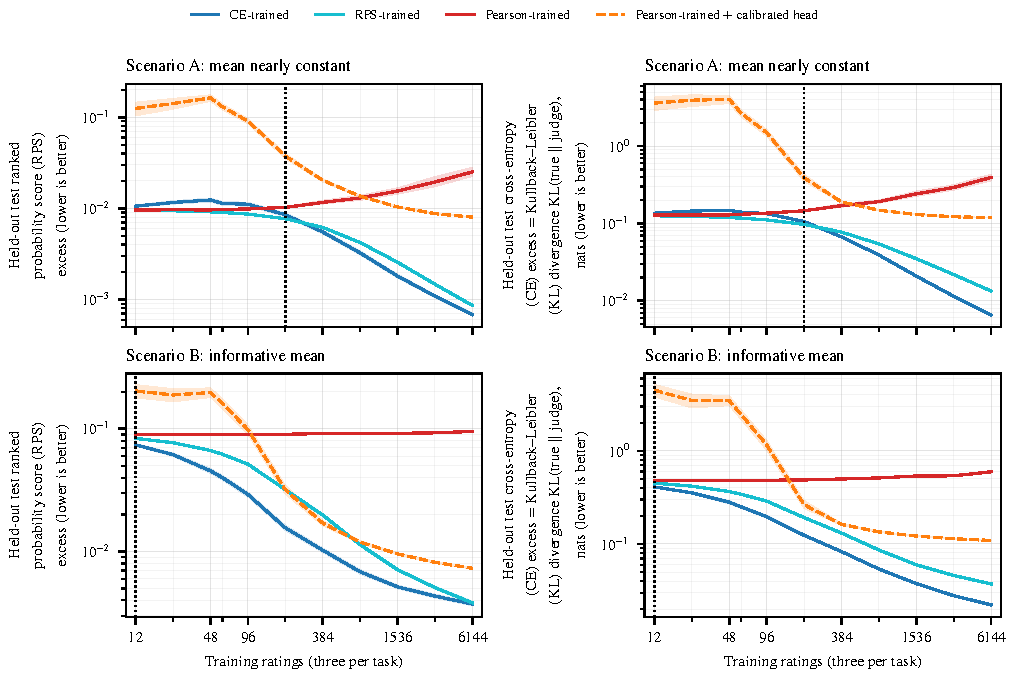
\includegraphics[width=0.96\textwidth]{figures/fig_exp13_curves.pdf}
\caption{\textbf{The CE-trained judge's error falls with more ratings, while the Pearson-trained judge's error stays flat or rises.}
Data: synthetic tasks with known rating distributions (experiment 13), 100 seeds per size, scored on 500 fresh tasks per seed.
Left column: held-out test ranked probability score (RPS) excess, the RPS of the forecast minus the RPS of the true distribution (0 is best; lower is better; log scale).
Right column: held-out test CE excess, $\mathrm{KL}(\text{true}\,\|\,\text{judge})$ in nats (0 is best; lower is better; log scale).
Horizontal axis: training ratings, three per task.
Rows: scenario A (nearly constant mean) and B (informative mean).
We chose each judge by L-BFGS-B (at most 400 iterations) from the training-histogram start with ridge weight $1/n$.
The CE objective is convex and the RPS and Pearson objectives are not, so their curves reflect this optimizer, start and budget.
Bands: 95\% percentile bootstrap intervals over seeds (10{,}000 draws).
Dotted vertical line: the smallest training size from which the CE-trained judge is significantly better than the Pearson-trained judge at every larger size (paired 95\% bootstrap lower bound above 0).}
\label{fig:exp13-curves}
\end{figure}

\begin{table}[t]
\caption{\textbf{The cross-entropy (CE)-trained judge's advantage grows with data in both scenarios, and is negative only in scenario A below 64 tasks.}
Held-out test ranked probability score (RPS) excess (0 is best; lower is better), mean over 100 seeds on 500 fresh tasks per seed.
The difference columns give the test RPS excess of the Pearson-trained judge minus that of the CE-trained judge, paired by seed, with a 95\% percentile bootstrap interval over seeds (10{,}000 draws); positive means the CE-trained judge is better.
We chose the judges as in \Cref{fig:exp13-curves}.}
\label{tab:exp13}
\centering\scriptsize
\setlength{\tabcolsep}{3pt}
\begin{tabular}{@{}rrrrrrr@{}}
\toprule
 & \multicolumn{3}{c}{Scenario A (mean nearly constant)} & \multicolumn{3}{c}{Scenario B (informative mean)} \\
\cmidrule(lr){2-4}\cmidrule(lr){5-7}
Tasks (ratings) & CE & Pearson & Pearson $-$ CE [95\% CI] & CE & Pearson & Pearson $-$ CE [95\% CI] \\
\midrule
4 (12) & 0.0106 & 0.0096 & -0.0010 [-0.0013, -0.0006] & 0.0740 & 0.0901 & +0.0161 [+0.0145, +0.0178] \\
8 (24) & 0.0116 & 0.0096 & -0.0020 [-0.0025, -0.0015] & 0.0616 & 0.0897 & +0.0281 [+0.0261, +0.0302] \\
16 (48) & 0.0123 & 0.0096 & -0.0027 [-0.0034, -0.0021] & 0.0454 & 0.0898 & +0.0444 [+0.0423, +0.0466] \\
32 (96) & 0.0111 & 0.0098 & -0.0013 [-0.0019, -0.0007] & 0.0292 & 0.0897 & +0.0606 [+0.0591, +0.0621] \\
64 (192) & 0.0085 & 0.0102 & +0.0017 [+0.0012, +0.0022] & 0.0156 & 0.0902 & +0.0747 [+0.0736, +0.0756] \\
128 (384) & 0.0055 & 0.0116 & +0.0061 [+0.0055, +0.0069] & 0.0102 & 0.0915 & +0.0813 [+0.0805, +0.0821] \\
2048 (6,144) & 0.0007 & 0.0251 & +0.0244 [+0.0217, +0.0277] & 0.0037 & 0.0951 & +0.0914 [+0.0894, +0.0936] \\
\bottomrule
\end{tabular}

\end{table}

\paragraph{A calibrated head does not close the gap.}
The Pearson-trained judge followed by a calibrated head never beats the CE-trained judge: its mean RPS excess is lower at none of the tested sizes.
It is far worse at small sizes, with RPS excess 0.1248 at 4 tasks in scenario A against 0.0106 for the CE-trained judge, and 0.2034 against 0.0740 in B.
The head beats the raw Pearson-trained judge (paired lower bound above 0 at every larger size) from 512 tasks (1{,}536 ratings) in A and from 64 tasks (192 ratings) in B.
At 2{,}048 tasks its RPS excess is 0.0080 in A and 0.0073 in B, against 0.0007 and 0.0037 for the CE-trained judge.
\Cref{fig:exp13-dist} shows why: where the mean is almost constant, the Pearson score barely varies, and one calibrated number cannot carry spread that it does not hold.
At $x=-0.7$ the raters split, and the true probability of the two extreme ratings is 0.66; the CE-trained judge assigns 0.62 and the calibrated head 0.34.
At $x=0$ the raters agree (0.08 on the extremes; CE-trained 0.07), and at $x=0.5$ they split again (0.51; CE-trained 0.53), yet the head assigns 0.34 at all three values.
The total variation distance to the true distribution is 0.07, 0.04 and 0.05 for the CE-trained judge against 0.32, 0.26 and 0.18 for the calibrated head.

\begin{figure}[t]
\centering
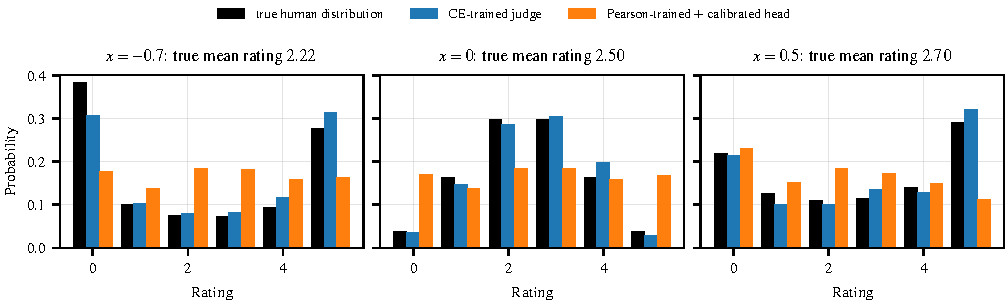
\includegraphics[width=0.96\textwidth]{figures/fig_exp13_distributions.pdf}
\caption{\textbf{The CE-trained judge recovers the split between ratings 0 and 5, and the calibrated Pearson score cannot.}
Data: scenario A of experiment 13 with 1{,}024 training tasks and three ratings per task, one illustrative training set drawn with a fixed random seed by \texttt{make\_memo\_assets.py} using experiment 13's code (not one of the 100 saved seeds).
Each panel shows one value of $x$ with a similar true mean rating (2.22, 2.50 and 2.70): black bars are the true human rating distribution, blue bars the CE-trained judge and orange bars the Pearson-trained judge with a calibrated head.
Vertical axis: probability of each rating.
We chose each judge by L-BFGS-B from the training-histogram start.
The CE objective is convex and the Pearson objective is not, so the orange bars reflect this optimizer, start and budget.}
\label{fig:exp13-dist}
\end{figure}

\paragraph{High correlation with a large distributional error, even without sampling noise.}
We also fit each objective on a dense 4{,}000-point grid of true distributions with near-zero ridge and the same optimizer and start, which removes sampling noise.
The same grid scores every fit, so each value in this paragraph is an in-sample numerical reference, not a held-out result or a proven large-sample limit, and the correlation fits are not certified optimal.
On the grid the Pearson-trained judge reaches Pearson correlation 0.9987 with the true mean in scenario A and 0.9988 in B, and its RPS excess is still 0.0872 and 0.0281.
The CE-trained judge has lower correlation (0.9395 and 0.9704) and far lower RPS excess (0.0003 and 0.0035).
With a calibrated head the Pearson-trained judge's RPS excess falls to 0.0072 and 0.0057 (correlation 0.9987 and 0.9946), which is still above the CE-trained judge's in both scenarios.

\subsection{Rank correlations and a Pearson--Spearman mix do not change the picture (experiment 06)}
\label{app:controlled-rank}

Experiment 06 trains the same 78-weight judge on the identical tasks, seeds and test tasks as experiment 13, with three further objectives. These are the Spearman correlation, Kendall's $\tau$ and the average of the Pearson and Spearman correlations between the judge's expected rating and the training-task mean ratings.
Rank correlations are not differentiable, so training uses smooth surrogates with temperature 0.1 rating points.
Refitting the CE-trained judge on the regenerated tasks (seed 0 in each of 22 scenario-by-size cells) reproduces experiment 13's saved RPS excess to within 7.6e-15.

In scenario B the CE-trained judge beats all four correlation-trained judges on test RPS excess from 4 tasks (12 ratings).
In scenario A it beats the Kendall-trained judge from 8 tasks (24 ratings) and the Pearson-trained, Spearman-trained and half-and-half judges from 64 tasks (192 ratings).
At 2{,}048 tasks the RPS excess of the correlation-trained judges is 8.8 to 25.5 times that of the CE-trained judge in B (0.0330 to 0.0951 against 0.0037) and 36.5 to 45.8 times in A (0.0249 to 0.0313 against 0.0007).
The half-and-half objective stays close to Pearson alone, so the tested equal-weight mix does not remove the distributional error (we did not test other weights), and the Kendall-trained judge has the largest RPS excess in A.

\begin{figure}[t]
\centering
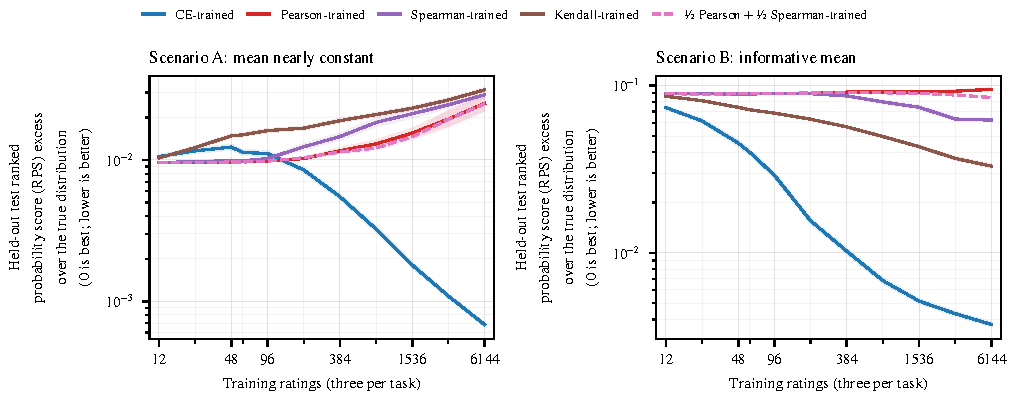
\includegraphics[width=0.96\textwidth]{figures/fig_exp06_rank.pdf}
\caption{\textbf{No tested correlation objective reaches the cross-entropy (CE)-trained judge's ranked probability score (RPS) excess, and in scenario A the rank objectives are worse than Pearson.}
Data: synthetic tasks with known distributions (experiments 06 and 13; identical training and test tasks), 100 seeds per size, 500 fresh test tasks per seed.
Vertical axis: held-out test RPS excess over the true distribution (0 is best; lower is better; log scale); horizontal axis: training ratings, three per task.
We chose each judge by L-BFGS-B (at most 400 iterations) from the training-histogram start with ridge weight $1/n$; rank objectives use smooth surrogates (temperature 0.1).
None of the correlation objectives is convex and we certified no fit, so these curves reflect this optimizer, start and budget.
Bands: 95\% percentile bootstrap intervals over seeds (10{,}000 draws).}
\label{fig:exp06-rank}
\end{figure}

\paragraph{Even on correlation, training on correlation buys little.}
In scenario A no correlation-trained judge has a higher mean test correlation than the CE-trained judge at any tested size, measured by Pearson correlation for the Pearson-trained and half-and-half judges and by Spearman correlation for the Spearman-trained and Kendall-trained judges (we did not evaluate Kendall's $\tau$ itself). At 2{,}048 tasks the CE-trained judge's test Pearson correlation with the true mean is 0.89, against 0.75 to 0.85 for the correlation-trained judges.
In scenario B the lead is just as wide at small sizes: at 16 tasks (48 ratings) the CE-trained judge's test Pearson correlation is 0.69, against 0.09 to 0.57 for the four correlation-trained judges.
The correlation-trained judges overtake on that correlation only with plenty of data.
In scenario B none has a higher mean correlation below 128 tasks.
In scenario B the differences become significant (paired lower bound above 0 at every larger size) from 256 tasks (768 ratings) for the Spearman-trained and Kendall-trained judges on test Spearman correlation, and from 512 tasks (1{,}536 ratings) for the Pearson-trained and half-and-half judges on test Pearson correlation.
In scenario B at 2{,}048 tasks the Spearman-trained judge's test Spearman correlation is 0.982 against 0.948 for the CE-trained judge, yet its RPS excess is 16.7 times as large.
A likely reason for the small-sample gap, which we did not test, is that the CE-trained judge learns from every rating, while a correlation-trained judge sees one noisy mean per task.

\subsection{The crossovers survive larger optimizer budgets and restarts (experiment 07)}
\label{app:controlled-budget}

Experiments 13 and 06 fit each judge once from one start, and the correlation objectives are not convex.
Experiment 07 reruns the same tasks (30 seeds, 4 to 1{,}024 training tasks) under three conditions.
The first is the original setting.
The second keeps the original start and raises the budget to 2{,}000 iterations and 4{,}000 function evaluations.
The third takes the best of five starts at that budget, chosen by the penalized training objective, so test data never enter the choice.
The CE reference has one start per budget, and we refit each calibrated head once on the selected Pearson score.

\begin{figure}[t]
\centering
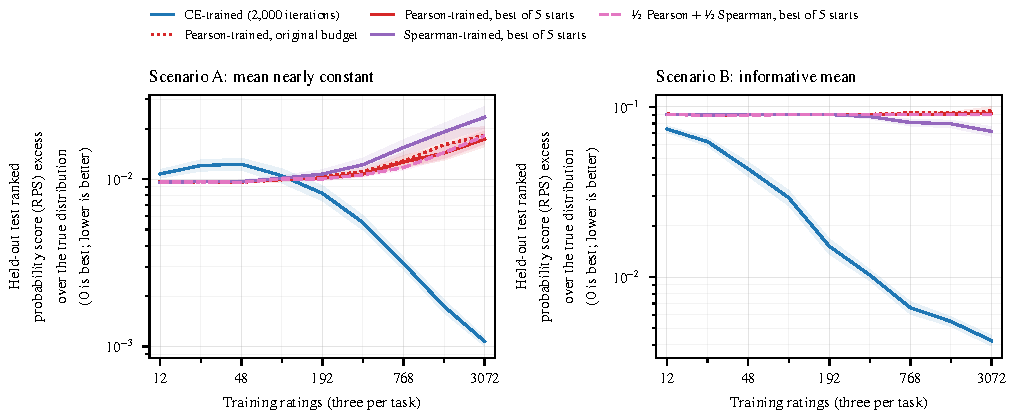
\includegraphics[width=0.96\textwidth]{figures/fig_exp07_restarts.pdf}
\caption{\textbf{Best-of-five restarts with a larger budget improve the correlation fits only slightly, and the CE-trained judge's lead remains.}
Data: synthetic tasks with known distributions (experiment 07), 30 seeds per size, 500 fresh test tasks per seed. Vertical axis: held-out test ranked probability score (RPS) excess over the true distribution (0 is best; lower is better; log scale); horizontal axis: training ratings, three per task.
Every curve has a 95\% percentile bootstrap band over seeds. Solid red and the solid Spearman-trained curve: the best of five starts (the original start and four random ones), each with 2{,}000 L-BFGS-B iterations and 4{,}000 function evaluations, chosen by the penalized training objective; dashed: the same for the half-and-half Pearson and Spearman objective. Dotted red: the original single Pearson start with 400 iterations. Solid blue: the CE-trained judge with one long start.
The CE objective is convex; the correlation objectives are not, and no global optimum was certified.
Bootstrap: 10{,}000 draws.}
\label{fig:exp07}
\end{figure}

\paragraph{The correlation fits rarely converge.}
From 32 training tasks on, the original-budget Pearson fits never converge, and 91\% of the long Pearson fits still hit the 2{,}000-iteration budget.
The half-and-half fits behave the same way (1\% converge at the original budget, and 89\% of the long fits hit the budget), and Spearman fits converge in 28\% at the original budget with 51\% of the long fits hitting it.
The CE-trained, RPS-trained and calibrated-head fits converge in 100\% of fits, and Kendall in 98\%.

\paragraph{Restarts improve the training objective, and the held-out RPS crossovers stay where they were.}
The best of five starts lowers the penalized training objective by more than $10^{-6}$ relative to the first long fit in 57\% to 90\% of the correlation fits (three objectives, nine sizes).
Yet at 1{,}024 tasks the RPS excess of the Pearson-trained judge barely moves. It goes from 0.0183 to 0.0173 in scenario A (CE-trained: 0.0011) and from 0.0949 to 0.0918 in scenario B (CE-trained: 0.0042).
Every crossover on held-out RPS excess is unchanged: 64 tasks (192 ratings) in A for Pearson, Spearman and the half-and-half mix, and 4 tasks (12 ratings) in B.
On held-out CE, only two scenario-A crossovers move, each by one grid step: the Spearman-trained judge's from 32 to 64 tasks and the Kendall-trained judge's from 32 to 16 tasks.
These checks test the optimizer budget and the start; they do not certify a global optimum for any correlation objective.

\paragraph{Numerical check of the cross-entropy gradient.}
A post-hoc review found that the frozen CE function of experiment 13 clips and renormalizes probabilities at $10^{-6}$ and returns an inconsistent gradient when clipping is active.
Refitting every CE judge with the exact objective and gradient leaves the reported results unchanged: in experiment 13 none of 2{,}200 rows differs by more than $10^{-9}$ in any metric, and in experiment 08 none of 4{,}400 fixed-ridge CE rows differs.
Of 4{,}400 validation-tuned CE rows in experiment 08, 338 move, by at most 0.00023 in RPS excess, and one ridge choice changes (the share choosing $c=0.01$ in scenario C at 256 tasks moves from 69\% to 68\%); all 95{,}291 exact-CE fits converged.
The saved Pearson rows came from another machine, which is a separate matter.
Rerunning the frozen code on the review machine reproduces the saved CE and RPS rows (none of 2{,}200 differs).
It does not reproduce the Pearson rows (2{,}198 of 2{,}200 differ, by up to 0.0082 in one row's RPS excess) or the calibrated heads fitted on them (2{,}198 differ, by up to 0.40).
We therefore treat each Pearson-trained curve as one realization of this optimizer and rely on the budget and restart checks above.

\subsection{Where the target's information lies matters more than its complexity (experiment 08)}
\label{app:controlled-complexity}

We fixed the hypothesis and the decision rule of experiment 08 before measuring.
The conjecture (ours, 11-13-2026) was that with little rating data a correlation-trained judge might work better, because it only has to get the mean right, so the number of ratings a CE-trained judge needs should grow with the complexity of the target.
Experiment 08 adds two scenarios with varying means and constant concentration: scenario C has the nonlinear mean of B with $\kappa=e^{1.5}$, and scenario D has the linear mean $\mu=0.5+0.35x$ with $\kappa=e^{1.5}$, the case most favorable to correlation.
Their variances still depend on the mean.
Every judge is experiment 13's softmax-linear model with the same optimizer.
The ridge weight is either fixed at $c=1$ or chosen from $\{0.01,0.1,1,10,100\}$ by four-fold cross-validation over the training tasks.
Cross-validation uses validation RPS for the CE-trained and RPS-trained judges, and validation Pearson correlation (or, as a further variant, validation RPS) for the tuned Pearson-trained judge.
A constant forecast of the training histogram serves as the baseline.
We use 100 seeds, 4 to 2{,}048 training tasks with three ratings each, and 500 fresh test tasks per seed.

\begin{table}[t]
\caption{\textbf{Correlation training wins at low data only in scenario A, where the mean says little; in B, C and D the cross-entropy (CE)-trained judge wins from 12 ratings.}
Experiment 08, held-out test ranked probability score (RPS) excess (0 is best; lower is better) on 500 fresh tasks per seed, 100 seeds.
First column of results: training ratings at which the Pearson-trained judge (fixed ridge) is significantly better than the CE-trained judge (paired 95\% bootstrap interval of the difference of test RPS excess entirely below 0).
Second: the smallest size from which the CE-trained judge (fixed ridge) is significantly better at every larger size.
Third: the same comparison between the validation-tuned CE-trained judge and the validation-tuned Pearson-trained judge.
Ratings are three per task.
We chose each judge by L-BFGS-B (at most 400 iterations) from the training-histogram start; the Pearson objective is not convex, so its results reflect this optimizer, start and budget.}
\label{tab:exp08}
\centering\small
\begin{tabular}{@{}p{0.27\columnwidth}p{0.17\columnwidth}p{0.17\columnwidth}p{0.17\columnwidth}@{}}
\toprule
Scenario & Pearson-trained better at & CE-trained better from & Tuned CE better from \\
\midrule
A: mean nearly constant, spread varies & 12 to 96 ratings & 192 ratings & 96 ratings \\
B: informative mean, spread varies & never & 12 ratings & 12 ratings \\
C: nonlinear mean, constant concentration & never & 12 ratings & 12 ratings \\
D: linear mean, constant concentration & never & 12 ratings & 48 ratings \\
\bottomrule
\end{tabular}

\end{table}

Neither hypothesis holds as stated (\Cref{tab:exp08}; \Cref{fig:ratings-needed} plots the four curves).
The low-data edge of correlation training appears only in scenario A, up to 96 ratings, and not in C or D, where the conjecture predicted it most strongly; the CE-trained judge needs the same 12 ratings in B, C and D.
On held-out correlation, the Pearson-trained judge (fixed ridge) overtakes the CE-trained judge only with plenty of data: from 512 tasks (1{,}536 ratings) in B and C and from 1{,}024 tasks (3{,}072 ratings) in D, and never in A.
Validation tuning is noisy with few tasks. Tuning both judges' ridge moves the crossover of scenario A from 64 to 32 tasks. The tuned CE-trained judge is significantly worse than the fixed-ridge Pearson-trained judge at 4, 8 and 16 tasks in A and at 4 tasks in D.
The Pearson-trained judge ends up worse than the constant forecast.
Its test RPS excess is significantly higher at every tested size from 128 tasks in A, 8 in B, 16 in C and 256 in D (paired 95\% lower bound above 0), and at 2{,}048 tasks the paired differences are +0.016, +0.028, +0.025 and +0.007.
Its held-out Pearson correlation with the true mean reaches 0.85, 0.99, 0.99 and 0.98.

What survives of the conjecture is narrow.
When the target's structure lies in higher moments and the mean carries little signal, a judge that matches the mean and keeps the average spread does well in small samples, and scenario A is consistent with that explanation, which we did not test directly.
What fails: in B, C and D the CE-trained judge has lower test RPS from the smallest tested size.
The ratings needed therefore depend on \emph{where} the target's information lies, not on its complexity alone: scenario B has A's varying disagreement plus an informative mean, and it crosses at 12 ratings.
Which scenario human ratings resemble is open.
On the human-rating sets of experiment 28 the Pearson fit has lower held-out RPS than the CE fit, by a simultaneous one-sided 97.5\% bound, in 19 of 325 cells: 18 at 10 ratings with five per item and one at 4 ratings with one per item (Section~\ref{sec:frozen}).
We did not test small-sample gains for correlation on other human ratings.

\subsection{Why correlation is the wrong primary metric}
\label{app:controlled-metric}

We give four reasons to report a proper score first and correlation second.
\begin{enumerate}
\item \textbf{Even on correlation, training on correlation buys little.} Below 128 training tasks no correlation-trained judge has a higher mean held-out correlation than the CE-trained judge, by the correlation reported for it (Pearson for the Pearson-trained and half-and-half judges, Spearman for the Spearman-trained and Kendall-trained judges), and in scenario A none does at any tested size. The correlation-trained judges overtake only with plenty of data in scenario B (\appref{app:controlled-rank}), while their rating distributions stay far worse (\Cref{fig:exp06-rank}).
\item \textbf{Correlation cannot see what matters.} Maximizing Pearson correlation minimizes the squared error between z-scored judge ratings and z-scored human ratings, so any shift or positive rescaling of the judge's ratings leaves it unchanged; these are exactly the bias and scale terms of squared error (\appref{app:moments-squared}). Any increasing transform leaves Spearman correlation unchanged. Both see one number per item, the mean, so neither identifies scale, signed bias or the pattern of rater disagreement. Correlation ties five different distributions in every replication of experiment 01. In experiment 00 (one seed, 2{,}000 synthetic human scores uniform on 0 to 5), a squashed judge that outputs only 4 or 5 has Pearson correlation 0.877 and Spearman correlation 0.878, against 0.900 and 0.900 for a noisy faithful judge. Its KL divergence to the human marginal histogram (Laplace-smoothed) is 3.420 nats, against 0.001 for the noisy faithful judge.
\item \textbf{Correlation is not a proper scoring rule.} It does not reward reporting the true rating distribution. Its value also depends on how spread out the test items are, not only on the judge, so one cannot average it item by item or compare it across test sets.
\item \textbf{What correlation is still good for.} If the only use is ranking items, Spearman correlation is a reasonable secondary diagnostic. To choose or train a judge that must reproduce human ratings, use a proper loss such as RPS and report correlations alongside it.
\end{enumerate}

\subsection{Retrospective comparison on theorem ratings}
\label{app:controlled-forest}

\Cref{fig:forest} summarizes the matched comparisons on the 75 theorem artifacts (25 tasks, 19 families, 195 expert ratings).
All of the studies reuse these ratings, so they are one body of evidence and not independent replications, and ``held out'' means held out from the fit, not from earlier judge selection.
For mixtures over five frontier judges no difference is established (experiment 02: $+0.0046$, 95\% interval $[-0.0100,+0.0356]$; archived experiment 12: $+0.0056$, $[-0.0059,+0.0181]$).
For the pool of 39 open-weight judges and the combined pool of 44 judges the CE-trained mixture is better ($+0.0502$, $[+0.0238,+0.0754]$; $+0.0405$, $[+0.0237,+0.0575]$).
The best single judge reverses the sign for the 44-judge pool, where selection by Pearson correlation is better ($-0.0317$, $[-0.0638,-0.0047]$), while selection by CE is better for the 39 open-weight judges ($+0.0529$, $[+0.0137,+0.0911]$), and no difference is established for the five frontier judges ($-0.0254$, $[-0.0570,+0.0005]$).
Each entry is the test RPS of the Pearson-trained judge minus that of the CE-trained judge; positive means the CE-trained judge is better.

\begin{figure}[t]
\centering
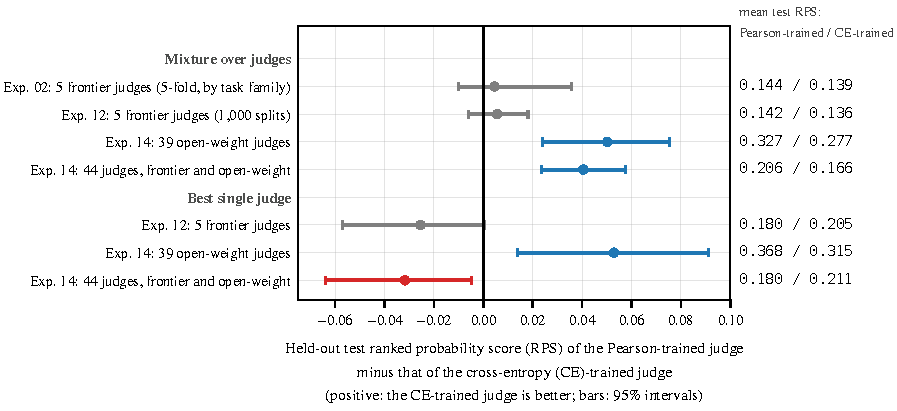
\includegraphics[width=0.82\textwidth]{figures/fig_forest.pdf}
\caption{\textbf{On the 75 retrospective theorem artifacts, the CE-trained mixture is better only for the larger judge pools, and selecting a single judge by Pearson correlation is better for the 44-judge pool.}
Data: held-out test artifacts from 25 tasks and 195 expert ratings, all used in earlier studies, so the comparison is retrospective and not a fresh test set.
Archived experiments 12 and 14 use 1{,}000 random splits with 20 training and 5 test tasks; experiment 02 uses five-fold task-family splits repeated over five partitions.
Horizontal axis: held-out test ranked probability score (RPS) of the Pearson-trained judge minus held-out test RPS of the CE-trained judge (0 means no difference; positive means the CE-trained judge is better; RPS ranges from 0 to 1 and lower is better).
Right column: mean test RPS of the Pearson-trained and the CE-trained judge.
Dots: mean differences; bars: 95\% percentile bootstrap intervals (10{,}000 draws over 25 tasks for archived experiments 12 and 14; 1{,}000 attempted task-family draws with refitting for experiment 02, of which 998 were usable).
Blue: CE-trained judge better; red: Pearson-trained judge better; gray: the interval includes 0.
Mixture weights over the base judges' rating histograms were fitted on the training tasks by an exact Pearson solver or by a convex CE solver with a suboptimality certificate, and single judges by exhaustive search over the pool (\appref{app:protocols}).}
\label{fig:forest}
\end{figure}

\section{The ranked probability score (RPS)}
\label{app:rps}
% Provenance: every worked-example number is printed by paper_latex_and_notes/AAAI_2027_EvalAIScientists_JudgesKL/rps_appendix_examples.py;
% make_memo_assets.py runs that script and logs its output in assets_log.txt. The archived-experiment-11 numbers come from
% experiments/archive/11_formulation4_train_only_ce_mixture_cv_start_10Nov2026_end_10Nov2026/results.md.

This appendix defines the ranked probability score (RPS), gives three ways to read it, proves that it is strictly proper, shows what it detects that mean-based metrics cannot, and states its limits.
RPS is not a standard machine-learning metric, so we write out every step.
A script prints every number below (\texttt{rps\_appendix\_examples.py}); the identities in this appendix hold to $2.2\times10^{-15}$ or better on random forecasts.

\subsection{Definition}
\label{app:rps-def}

A human rating is an ordered category $r\in\{0,1,\dots,5\}$.
For an item, a judge outputs a forecast $q=(q_0,\dots,q_5)$.
Its cumulative distribution function (CDF) and survival function are
\begin{equation}
Q_j=\Pr_q[R\le j]=\sum_{k=0}^{j}q_k,\qquad S_j=\Pr_q[R>j]=1-Q_j,\qquad j=0,\dots,4 .
\end{equation}
We omit the threshold $j=5$ because $Q_5=1$ for every forecast.
The ranked probability score~\citep{epstein1969scoring} compares the judge's CDF with the step function of the observed rating:
\begin{align}
L_{\RPS}(q,r)&=\frac15\sum_{j=0}^{4}\bigl(Q_j-\Ind\{r\le j\}\bigr)^2 \label{eq:rps-cdf}\\
&=\frac15\sum_{j=0}^{4}\bigl(S_j-\Ind\{r>j\}\bigr)^2 .\label{eq:rps-sf}
\end{align}
We use it as a loss: lower is better.
Dividing by the five thresholds puts it in $[0,1]$.
It equals 0 when $q$ puts all its mass on $r$, and it equals 1 when $q$ puts all its mass on the opposite end of the scale (a point mass on rating 0 scored against a rating of 5).
Some references omit the factor $1/5$, and their values are five times ours.

For $N$ items $x_i$ with $n_i$ human ratings $r_{i1},\dots,r_{in_i}$ each, we average over the ratings of an item and then over items:
\begin{equation}
\widehat{\RPS}=\frac1N\sum_{i=1}^{N}\frac1{n_i}\sum_{m=1}^{n_i}L_{\RPS}(q_i,r_{im}).
\end{equation}
Writing $\hat P_{ij}$ for the empirical CDF of item $i$'s ratings, the inner average equals $\frac15\sum_j\bigl[(Q_{ij}-\hat P_{ij})^2+\hat P_{ij}(1-\hat P_{ij})\bigr]$.
A single rating per item already gives an unbiased estimate of the judge's expected score, so we estimate no per-item histogram.

\subsection{Three ways to read RPS}
\label{app:rps-read}

\paragraph{Five yes/no questions.}
At each threshold $j$ the judge answers ``is the rating at most $j$?'' with probability $Q_j$, and the human rating supplies the answer.
Each summand in \Cref{eq:rps-cdf} is the Brier score of one such binary forecast, so RPS is the average Brier score over the five threshold questions.
Equation~\ref{eq:rps-sf} says the same for the chance that the rating exceeds each threshold.

\paragraph{Distance between staircases.}
The judge's CDF is a staircase that rises from 0 to 1, and the observed rating is a single step at $r$.
RPS sums the squared vertical gaps between the two staircases, so a near miss leaves gaps at few thresholds and a far miss at many.
\Cref{fig:rps-staircase} works one example: for the forecast $q=(0,0,0.1,0.3,0.4,0.2)$ and the rating $r=4$, the cumulative probabilities are $Q=(0,0,0.1,0.4,0.8)$, the squared gaps are $(0,0,0.01,0.16,0.04)$ and RPS is $0.21/5=0.042$.
\Cref{tab:rps-examples} compares four forecasts against the same rating.
Cross-entropy (CE) is infinite for every forecast with $q_4=0$, and the categorical Brier score $\sum_k(q_k-\Ind\{r=k\})^2$ equals 2 for every point mass away from 4.
Only RPS scores the near miss (all mass on rating 5, RPS 0.200) better than the far miss (all mass on rating 0, RPS 0.800).
A point mass $d$ ratings away from the observed rating scores $d/5$: 0.0, 0.2, 0.4, 0.6 and 0.8 for $d=0,\dots,4$.

\begin{figure}[t]
\centering
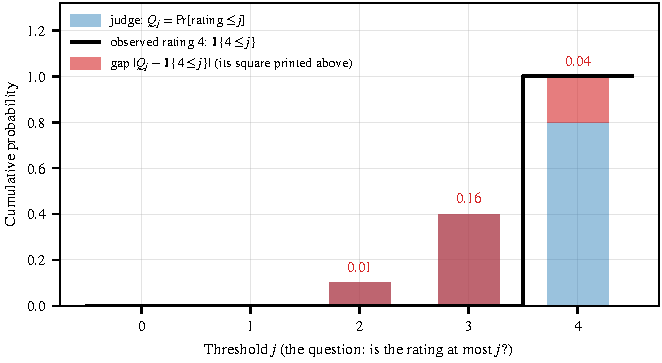
\includegraphics[width=0.62\textwidth]{figures/fig_rps_staircase.pdf}
\caption{\textbf{RPS adds the squared gaps between the judge's cumulative probabilities and the observed rating's step.}
Constructed example, not data: the judge's forecast over ratings 0 to 5 is $(0,0,0.1,0.3,0.4,0.2)$ and the human rating is 4.
Horizontal axis: the five thresholds $j$; vertical axis: cumulative probability.
Blue bars: the judge's $Q_j=\Pr[\text{rating}\le j]$; black staircase: the observed rating's step $\Ind\{4\le j\}$; red: the gap, with its square printed above.
RPS $=(0.01+0.16+0.04)/5=0.042$ (range 0 to 1, lower is better; a perfect forecast scores 0).}
\label{fig:rps-staircase}
\end{figure}

\begin{table}[t]
\caption{\textbf{Only RPS scores a near miss better than a far miss.}
Scores of four forecasts against one human rating $r=4$ (lower is better for all three scores).
RPS: ranked probability score, range 0 to 1.
Brier: categorical Brier score $\sum_k(q_k-\Ind\{r=k\})^2$, range 0 to 2.
CE: cross-entropy $-\log q_4$ in nats, infinite when $q_4=0$.}
\label{tab:rps-examples}
\centering\small
\begin{tabular}{lccc}
\toprule
Forecast for $r=4$ & RPS & Brier & CE \\
\midrule
all mass on 4 & 0.000 & 0.0 & 0 \\
all mass on 5 & 0.200 & 2.0 & $\infty$ \\
all mass on 0 & 0.800 & 2.0 & $\infty$ \\
half on 3, half on 5 & 0.100 & 1.5 & $\infty$ \\
\bottomrule
\end{tabular}
\end{table}

\paragraph{Rating points.}
For integer ratings, RPS has an absolute-error form, the discrete case of the identity for the continuous ranked probability score~\citep{matheson1976scoring,gneiting2007strictly}:
\begin{equation}
5\,L_{\RPS}(q,r)=\E_q|R-r|-\tfrac12\E_q|R-R'| ,
\label{eq:rps-abs}
\end{equation}
where $R$ and $R'$ are independent draws from $q$.
The first term is the expected distance, in rating points, between a rating sampled from the judge and the human rating.
The second term subtracts half of the judge's own spread, so the score does not penalize a judge merely for spreading its probability.
To see \Cref{eq:rps-abs}, write $|a-r|=\sum_{j=0}^{4}\bigl|\Ind\{a\le j\}-\Ind\{r\le j\}\bigr|$ for integers $a$ and $r$; taking the expectation over $a\sim q$ gives $\E_q|R-r|=\sum_j[Q_j+o_j(1-2Q_j)]$ with $o_j=\Ind\{r\le j\}$, and $\E_q|R-R'|=2\sum_jQ_j(1-Q_j)$, so the right-hand side of \Cref{eq:rps-abs} equals $\sum_j(Q_j-o_j)^2$ because $o_j^2=o_j$.

\subsection{RPS is strictly proper}
\label{app:rps-proper}

Let the human rating be drawn from $p$ with CDF $P$.
Then, for each threshold, $\E[(Q_j-\Ind\{R\le j\})^2]=Q_j^2-2Q_jP_j+P_j=(Q_j-P_j)^2+P_j(1-P_j)$, and summing over the thresholds gives
\begin{equation}
\E_{R\sim p}\bigl[L_{\RPS}(q,R)\bigr]=\underbrace{\frac15\sum_{j=0}^{4}(Q_j-P_j)^2}_{\text{excess: the judge's error}}+\underbrace{\frac15\sum_{j=0}^{4}P_j(1-P_j)}_{\text{rater disagreement}} .
\label{eq:rps-decomposition}
\end{equation}
The second term does not depend on $q$: it is the irreducible disagreement among raters.
The first term is nonnegative, and it vanishes only when $Q_j=P_j$ at every threshold, that is, when $q=p$.
So RPS is strictly proper~\citep{gneiting2007strictly}: a judge minimizes its expected RPS only by reporting the full human rating distribution, including how much the raters disagree.
The script checks \Cref{eq:rps-abs,eq:rps-decomposition} on 2{,}000 random forecasts and distributions, with a maximum absolute error of $1.8\times10^{-15}$.

\subsection{What mean-based metrics miss}
\label{app:rps-mean}

\paragraph{An example of disagreement that correlation cannot see.}
Suppose raters split evenly between ratings 3 and 5 on an item.
Judge~A forecasts the human distribution, and judge~B puts all its mass on rating 4.
Both have expected rating 4.0, so replacing one forecast by the other cannot change a correlation computed from expected ratings across a panel of items; if all expected ratings are constant, the correlation is undefined for both judges.
Judge~A has expected RPS 0.10, which is all irreducible disagreement, whereas judge~B has 0.20.
A uniform forecast over ratings 0 to 5 scores 0.206.

\paragraph{The mean is the sum of the survival function.}
For ratings in $\{0,\dots,5\}$,
\begin{equation}
\E_q[R]=\sum_{j=0}^{4}\Pr_q[R>j]=\sum_{j=0}^{4}S_j .
\label{eq:mean-survival}
\end{equation}
Mean squared error between expected ratings depends on a forecast only through this sum, and correlation across items is weaker still, because shifting or positively rescaling the sums leaves it unchanged.
Survival gaps of opposite sign at different thresholds therefore cancel in every mean-based metric.
RPS squares the gap at each threshold before adding, so the gaps cannot cancel.
In the example, judge~A has $S=(1,1,1,0.5,0.5)$ and judge~B has $S=(1,1,1,1,0)$.
Both sum to 4, so their gaps $(0,0,0,+0.5,-0.5)$ cancel in the mean, while their squares give the excess expected RPS $(0.25+0.25)/5=0.10$.
The script checks \Cref{eq:mean-survival} on 1{,}000 random forecasts, with a maximum absolute error of $2.2\times10^{-15}$.

\subsection{Why the cumulative form: scoring with a few ratings per item}
\label{app:rps-sparse}

Each item has two or three human ratings in our retrospective studies, so its empirical histogram leaves at least three of the six bins empty.
For a forecast that gives positive mass to an unobserved rating, the Kullback--Leibler (KL) divergence $\KL(q\|\hat p)$ from the empirical histogram $\hat p$ is infinite unless we smooth $\hat p$.
The reverse direction, $\KL(\hat p\|q)$, is finite whenever $q$ is positive on the observed ratings, and it differs from the empirical CE by a term that does not depend on the judge (the entropy of $\hat p$).
Empty empirical bins therefore do not invalidate individual-rating CE or the categorical Brier score.

Plug-in distances to a histogram of one to three ratings are a different matter.
Total variation distance (TVD) is biased upward even for the true distribution.
Suppose raters choose rating 3 with probability 0.6 and rating 5 with probability 0.4.
The true distribution's expected TVD to its own histogram of 1, 2 or 3 ratings is 0.48, 0.288 and 0.23.
With one rating per item, a forecast that puts all its mass on 3 scores better than the truth (\Cref{tab:rps-sparse}), so plug-in TVD rewards overconfidence.
The one-rating Wasserstein-1 distance, the summed absolute gap between the CDFs, has the same flaw, because a point mass at the median minimizes it.
RPS ranks the truth first.

\begin{table}[t]
\caption{\textbf{With one rating per item, plug-in TVD and Wasserstein-1 prefer the overconfident forecast to the true distribution, and RPS does not.}
Raters choose rating 3 with probability 0.6 and rating 5 with probability 0.4 (constructed example, not data).
The first two columns score each forecast against a histogram of one sampled rating, averaged over that rating's distribution: TVD is total variation distance (range 0 to 1) and W1 is the Wasserstein-1 distance (rating points).
The last column is the expected RPS (range 0 to 1).
Lower is better in every column, and the truth is the only forecast that a proper score must rank first.}
\label{tab:rps-sparse}
\centering\small
\begin{tabular}{lccc}
\toprule
Forecast & one-rating TVD & one-rating W1 & expected RPS \\
\midrule
truth ($0.6$ on 3, $0.4$ on 5) & 0.48 & 0.96 & 0.096 \\
all mass on 3 & 0.40 & 0.80 & 0.160 \\
all mass on 4 & 1.00 & 1.00 & 0.200 \\
\bottomrule
\end{tabular}
\end{table}

RPS avoids this improper plug-in comparison by scoring each observed rating, because every rating supplies a binary answer at every threshold, even when an empirical CDF equals 0 or 1.
With $n$ independent ratings of an item, $\hat P_{ij}$ is unbiased for $P_{ij}$ and has variance $P_{ij}(1-P_{ij})/n$: at $P_{ij}=0.6$ this is 0.240, 0.120 and 0.080 for $n=1,2,3$.
The expected empirical threshold floor $\hat P_{ij}(1-\hat P_{ij})$ is $(1-1/n)P_{ij}(1-P_{ij})$, which is 0.000, 0.120 and 0.160, so a plug-in estimate of the floor depends on $n$.
Averaging the individual-rating scores instead keeps the full disagreement term of \Cref{eq:rps-decomposition} for every $n$ (0.096 in this example for $n=1,2,3$).
That term cancels in expected differences between judges, and observed paired differences still carry sampling noise.

\subsection{RPS as a distance, and ``root RPS''}
\label{app:rps-distance}

If we knew the human distribution $p$, the excess term of \Cref{eq:rps-decomposition} would be $\frac15\sum_j(Q_j-P_j)^2$, one fifth of the squared $\ell_2$ distance between the two CDFs on the integer scale.
The $\ell_2$ distance between CDFs is the Cramér distance of \citet{bellemare2017cramer}, so $\sqrt{5\times\text{excess}}$ is a Cramér distance.
On this scale the excess also equals one tenth of the energy distance $2\E|X-Y|-\E|X-X'|-\E|Y-Y'|$ for independent draws from $q$ and $p$~\citep{szekely2013energy}; the script checks this to $2.2\times10^{-15}$.
The square root of the excess is a true metric between rating distributions, a principled ``root RPS''.
In practice $p$ is unknown.
With one rating per item and no further assumptions we cannot separate the excess from the disagreement floor, but the floor is the same for every judge.
Differences in mean RPS between two judges are therefore unbiased estimates of the differences in their squared CDF gaps to the human distributions, scaled by $\frac15$.
Here ``root RPS'' means the square root of the excess, not of the observed individual-rating loss: taking the square root of a mean RPS leaves the ranking of judges unchanged, but taking it per rating before averaging would lose the unbiasedness.
\citet{bellemare2017cramer} also show that, unlike the Wasserstein distance, the Cramér distance has unbiased sample gradients, which makes RPS usable as a training loss as well as an evaluation metric.

\subsection{Why RPS is the primary metric for ordinal human ratings}
\label{app:rps-why}

We use RPS as the primary and common selection metric of the prospective evaluation, for five reasons.
\begin{enumerate}
\item \textbf{Order matters.} Ratings are ordered, and RPS charges more for larger misses, while CE and the categorical Brier score treat ratings as unordered labels.
\item \textbf{It targets the whole distribution.} RPS is strictly proper (\appref{app:rps-proper}), so only the true conditional rating distribution minimizes it. Correlation ignores calibration and spread, and mean squared error identifies only the conditional mean (\Cref{app:rps-mean}).
\item \textbf{It works with sparse ratings.} Each observed rating is scored directly through the CDF, so items with one to three ratings contribute without a histogram estimate, and empty rating categories do not distort the score (\appref{app:rps-sparse}).
\item \textbf{It is bounded.} RPS lies in $[0,1]$, so a single rating that received near-zero probability cannot dominate it. CE can be dominated this way. In archived experiment 11 (75 theorem artifacts from 25 tasks; repeated five-fold task-grouped cross-validation with 20 repeats; out-of-fold scores), the CE-trained mixture of judges has higher out-of-fold CE than a constant forecast of the training ratings: 5.427 against 1.848 nats (lower is better). The $10^{-6}$ probability floor dominates CE on histograms of three ratings. Yet the mixture's out-of-fold RPS is lower, 0.1367 against 0.1829. The paired difference of out-of-fold RPS, the CE-trained mixture minus the constant forecast, is $-0.0462$ (95\% task-bootstrap interval $[-0.0937,-0.0005]$, 10{,}000 draws); negative favors the mixture.
\item \textbf{It is interpretable.} The absolute-error form (\Cref{eq:rps-abs}) is in rating points, and \Cref{eq:rps-decomposition} separates the judge's error from the noise floor set by rater disagreement.
\end{enumerate}

\subsection{Limitations}
\label{app:rps-limits}

RPS assumes equally spaced ratings: a miss from 0 to 1 costs the same as a miss from 4 to 5.
It weights all thresholds equally.
It is less sensitive than CE to the probability that a forecast gives to rare ratings, which is why we keep CE as a secondary metric.
With $n_i>1$ independent ratings, $\frac{n_i}{n_i-1}\hat P_{ij}(1-\hat P_{ij})$ is an unbiased but noisy estimate of the disagreement at a threshold, so we compare judges by paired differences on the same items.

\citet{galdran2023performance} notes two further behaviors.
First, the penalty for a confident miss grows only linearly with distance, as the values $d/5$ above show.
Second, RPS can prefer a symmetric forecast to one with more probability on the observed rating.
That work proposes a squared-absolute variant, $\frac15\bigl(\sum_j|Q_j-\Ind\{r\le j\}|\bigr)^2$.
In our numerical check the variant is not proper: for raters distributed $(0.2,0.2,0.2,0.2,0.1,0.1)$ over ratings 0 to 5, the forecast $(0,0,0.9,0.1,0,0)$ has a lower expected variant score (0.498) than the true distribution (0.680), whereas RPS prefers the truth (0.178 against 0.246).
We therefore keep RPS.

\section{Metric and protocol definitions}
\label{app:protocols}

\paragraph{Metrics.}
For a forecast $q$ on $K$ ordered categories and an individual rating $y$:
normalized RPS $=\frac1{K-1}\sum_{k=0}^{K-2}(F_q(k)-\mathbf 1\{y\le k\})^2\in[0,1]$ (lower is better; the RPS of the uniform forecast depends on the human distribution and is listed beside each result);
CE $=-\log q(y)$ in nats (the uniform forecast scores $\log K$: $0.693$, $1.099$, $1.609$, $1.792$ for $K=2,3,5,6$);
TVD $=\tfrac12\sum_r|h(r)-q(r)|$ against the item's empirical human distribution $h$ (0--1), averaged equally over items;
Brier $=\sum_r(q(r)-\mathbf 1\{y=r\})^2\in[0,2]$;
normalized mean squared error is the mean of $((m-y)/(K-1))^2$.
Scores are averaged over the individual ratings of an item and then equally over items.
Pearson, Spearman and Kendall correlations are computed across items between the expected score of the forecast and the mean human rating.
A probability floor $q\leftarrow(1-K\epsilon)q+\epsilon$ with $\epsilon=10^{-6}$ is applied before CE unless stated (experiment 25 uses $6\times10^{-6}$ for test CE; experiment 16 sweeps $10^{-6}$ to $5\times10^{-2}$).
An all-undefined Pearson fit (every candidate gives a constant score, as with two distinct training means) keeps the identity setting.

\paragraph{Differences.}
Every difference subtracts the same metric on the same data for two procedures named by how they were trained, and says which sign favors which.
In particular ``test RPS of the Pearson-trained judge minus test RPS of the CE-trained judge'' is positive when the CE-trained judge is better.

\begin{table*}[t]
\caption{\textbf{Protocols by experiment family.}
Every study uses the same two-judge design: identical except for the training objective, with the same training ratings, the same search space and the same test items.
Intervals: simultaneous (maximum-$t$) one-sided or two-sided bands as stated; ``crossed'' bands resample training draws and held-out units together, ``conditional'' bands condition on the matched training draws.
Frozen protocols and hashes are in each experiment folder.}
\label{tab:protocols}
\centering\scriptsize
\setlength{\tabcolsep}{3pt}
\begin{tabular}{@{}p{0.08\textwidth}p{0.22\textwidth}p{0.23\textwidth}p{0.19\textwidth}p{0.21\textwidth}@{}}
\toprule
Experiments & Data and test unit & Fit and search & Budgets and draws & Intervals \\
\midrule
01 & Synthetic, 96 train / 48 validation / 48 test items; exact test scoring & Nine fixed candidates, exhaustive selection on validation ratings & 1, 2 or 3 ratings per validation item; 256 draws & Student-$t$ 95\% over draws \\
04, 05 & Synthetic populations (11 artifacts); exact expectations & Closed-form forecasts; exact rational vertex enumeration for the worst case; REML for design allocation (Phase B) & Phase B: 256 replications; A1 finite sample 4{,}000 & Student-$t$ 95\%; Wilson 95\% for counts; no $p$-values \\
06, 07, 08, 11, 13, 17 & Synthetic judges on known distributions (scenarios A--D); fresh test tasks scored against the truth & L-BFGS-B with 400 iterations; experiment 07: 5$\times$ budget and best of five starts; validation-tuned ridge (08, 11) & 4 to 2{,}048 tasks; seeds as in each folder & Over seeds \\
18, 20 & Synthetic (6 features, softmax-linear) and the 75 retrospective artifacts (task-grouped splits) & Same head and optimizer, only the objective differs; heads on judge scores; single-judge selection & Synthetic 4 to 512 items, 200 seeds (20); sweeps of 252 cells (18); 400 real splits & 95\% over seeds (synthetic); see folders for real-data intervals \\
02, 12, 14, 16, 19 & 75 artifacts, 25 tasks, 19 families, 195 expert ratings; task-family folds & Simplex mixtures (SLSQP with a Frank--Wolfe certificate for CE; exhaustive faces for Pearson); single-judge picks & 5 partitions $\times$ 5 folds (02); 1{,}000 task-grouped 20/5 splits (12, 14, 16) & Task-family bootstrap, 1{,}000 draws, 95\% percentile (02); see folders for the others \\
21, 26 & 160 homework answers, 67 questions, two graders; one 16-answer assignment held out per fold & 27-setting head, exhaustive, ties to the identity setting; CE, Pearson, training histogram, uniform & 4 to 256 ratings, 2 per answer (and 1 per answer); 200 draws per assignment & Overlap-adjusted paired $t$ over ten assignments; descending test at level 0.01 \\
23 & SummEval (40 articles, 1{,}920 grades), KonIQ-10k (2{,}015 held-out images, 215{,}415 votes), dialogue, MovieLens & 27 or 216 candidate forecasts, exhaustive; CE, Pearson, RPS fits and calibrated comparators & 6 to 768 (SummEval), 6 to 6{,}144 (KonIQ); 64 matched draws & Simultaneous 97.5\% bands; 4{,}000 bootstraps of articles or images \\
28 & ChaosNLI (SNLI 600, MNLI-matched 600, alphaNLI 400 items; 100 labels) and DICES (350 and 400 items); five frontier judges & 27-setting head, exhaustive, ties to the identity setting & 4 to 256 ratings (1 per item) and 10 to 320 (5 per item); 200 draws per fold & Simultaneous one-sided 97.5\%, 4{,}000 bootstrap of held-out items \\
24, 25, 29 & HelpSteer2 (1{,}038 responses, 519 prompts), ChaosNLI, DICES, alphaNLI & LoRA (rank 8, $\alpha=16$, top four blocks), AdamW, learning-rate grid, validation-RPS checkpoint; 1D or $(K+2)$ logit calibration & 16 to 8{,}192 total ratings; 10 or 20 nested draws & Simultaneous max-$t$ 95\%, 4{,}000 draws, conditional and crossed \\
31 & Saved results of 26, 28 and 29 & Weighted least squares over a 150-value grid of $b\in[0.02,3]$ & 2{,}000 parametric bootstrap draws per curve & Percentile 95\% \\
\bottomrule
\end{tabular}
\end{table*}

\paragraph{How each judge was chosen.}
For frozen judges the fit is an exhaustive search over a finite family (27 calibration settings; 216 candidate distributions for KonIQ). It returns the exact optimum of the stated objective within that family, with ties broken toward the setting nearest the identity. For the mixture fits of experiment 02 the CE objective is convex and certified by a Frank--Wolfe gap of at most $10^{-8}$. The Pearson objective is solved exactly on every face of the cone, with a cone-projection certificate.
For trained judges (toy softmax models and LoRA) the objectives are optimized by L-BFGS-B or AdamW from a fixed start; Pearson objectives are not convex and the result reflects that optimizer, start and budget, and not a certified global optimum.
Model-selection data are never the test data.

\section{Index of all experiments}
\label{app:index}

\Cref{tab:index} lists every experiment folder of the repository: 30 active folders and the four archived experiments 11--14, as of 11-25-2026.
Dates are the day each folder was started (2026, month-day, America/Los\_Angeles).
The headline column states the data and metric of the result; ``retro.'' marks studies on the 75 retrospective theorem artifacts and 195 expert ratings.
Unless a row says otherwise, a signed difference is the held-out test RPS of the Pearson-trained judge minus that of the CE-trained judge, so positive values favor CE.
Two folders carry the number 11, one active and one archived. Experiment 32 was created as a second experiment 30 and was renumbered on 11-25-2026 under the repository's duplicate-number rule.

{\small
\begin{longtable}{@{}p{0.045\textwidth}p{0.05\textwidth}p{0.25\textwidth}p{0.55\textwidth}@{}}
\caption{\textbf{Experiment index.} Metrics are held-out unless marked synthetic or exact; differences name the procedures and the favored sign.}\label{tab:index}\\
\toprule
Exp. & Start & Question & Headline result \\
\midrule
\endfirsthead
\toprule
Exp. & Start & Question & Headline result \\
\midrule
\endhead
\bottomrule
\endfoot
00 & 11-07 & Can a squashed judge look good under correlation? & Two synthetic judges on 2{,}000 scores, no fitting: noisy-faithful Pearson $0.900$, KL $0.001$; squashed Pearson $0.877$, KL $3.420$ (marginal histograms); one seed. \\
01 & 11-08 & Which criteria identify a known conditional distribution among nine candidates? & CE chose the true distribution in 249/256 draws with one rating per item, Brier and RPS in 245/256, all in 256/256 with two or three ratings; Pearson, Spearman, Kendall and scaled squared error always tied the five same-mean candidates. \\
02 & 11-09 & Matched CE versus Pearson mixtures on the retro.\ ratings & Test CE of the CE-trained minus Pearson-trained mixture $-0.260$ nats ($[-1.458,+0.198]$; negative favors CE); test RPS $0.139$ (CE-trained), $0.144$ (Pearson-trained), constant forecast $0.187$. \\
04 & 11-13 & Are reliability and moment matching enough for distribution accuracy? & No: equal mean, variance and reliability give mean TVD $0.446$ and excess RPS $0.0167$; the most repeatable historical judge had the worst test RPS; decision-study allocation chose the best design in 256/256 replications in each of two configurations. \\
05 & 11-13 & How big is the information gap between CE and correlation? & Mean-only (maximum-entropy) forecast pays $0.117$ nats on average (item range $0.020$ to $0.210$); three Pearson-1 forecasts differ by $0.117$ to $3.635$ nats of KL. \\
06 & 11-13 & Do rank or mixed correlation objectives fix Pearson? & CE-trained beats Pearson, Spearman, Kendall and half-and-half judges on held-out RPS and CE from 12 ratings (scenario B) and 192 ratings (scenario A); synthetic. \\
07 & 11-13 & Do optimizer budget and restarts change experiments 06 and 13? & No held-out RPS crossover changes; best of five starts improves the training objective in 57--90\% of correlation fits. \\
08 & 11-14 & Does correlation win with little data when the mean is informative? & CE-trained better from 12 ratings in scenarios B, C, D; Pearson-trained better up to 96 ratings only in scenario A (uninformative mean). \\
09 & 11-16 & Open-weight judges: native probabilities, prompt, harness and LoRA optimization & Native six-category CE $1.629$ nats against $3.480$ for scalar votes, constant $1.887$; proper-loss optimization beat correlation optimization in all three layers; retro. \\
10 & 11-16 & Frontier judges: native probabilities and prompt search & Native CE $1.416$ against $5.49$ nats, constant $1.928$; 15-judge mixture, test RPS of the Pearson-trained minus CE-trained $+0.0775$ ($[+0.0437,+0.1135]$); single prompt or harness selection uncertain; retro. \\
11 & 11-17 & Tuned heads and squared-error training against CE (toy) & Cross-fitted heads cut the small-sample spike 3--9$\times$; end-to-end CE dominates when disagreement varies (scenarios A, B); excess CE $0.118$--$0.197$ nats for squared error against $0.0066$--$0.0224$. \\
15 & 11-20 & Rater severity versus item signal & Offsets $\approx0.1$ points, $\approx2\%$ of within-artifact variance; rankings unchanged (Kendall $\tau\ge0.995$); retro. \\
16 & 11-20 & RPS-selected judge and probability-floor sweep & Picking one judge by RPS is no better than by CE or correlation; RPS-selected mixtures are the best fitted arm; floor lowers selected-CE from $8.9$ to $2.2$ but not below the constant; retro. \\
17 & 11-20 & Is a scalar score a bottleneck? & Flexible head on the true mean matches or beats CE from 512 items; with a Pearson-learned score a gap remains in scenario A: test RPS of the Pearson-trained score with a flexible head minus that of the end-to-end CE-trained judge is $+0.0052$ at 2{,}048 items; synthetic. \\
18 & 11-21 & When does CE beat correlation? & Crossover 16, 32, 64 items with 10, 3, 1 ratings per item; Pearson-then-calibrate wins when spread follows the mean; on a 44-judge pool the Pearson-trained minus the CE-trained mixture is $+0.048$ to $+0.090$ test RPS; single-judge Pearson as good or better. \\
19 & 11-21 & Moment recovery with few ratings & Qwen pair had lower RPS after CE than Pearson fitting at about 12 ratings; uniform beat both Qwen fits; closed pair unresolved; retro. \\
20 & 11-21 & CE- versus Pearson-trained judge with little data & RPS excess of the Pearson-trained minus the CE-trained judge $+0.034$ at 16 items (48 ratings; $[0.031,0.036]$) and $-0.027$ at 4 items; on the retro.\ ratings a CE-trained head beats a Pearson-trained head by $+0.035$ to $+0.058$ test RPS from 7 training families in the closed-weight and all-59 judge pools; synthetic and retro. \\
21 & 11-21 & Fresh task families, two frozen judges (homework) & Qwen3.5-9B: CE-fit RPS $0.1548$ against $0.2263$ at 4 ratings, passes at all seven budgets; Claude Sonnet 5 never passes; two graders, ten folds. \\
22 & 11-21 & Non-circular evaluation protocol & No runs: held-out RPS first, metrics neither objective optimizes, public-set shortlist (ChaosNLI, DICES, HelpSteer2). \\
23 & 11-21 & Public ordinal ratings and label cost & KonIQ: CE beats raw Pearson and uniform from 12 ratings, no sustained win over all four controls; SummEval and MovieLens: none; dialogue: calibrated Pearson lower. \\
24 & 11-21 & LoRA judge on HelpSteer2 & Test RPS of the calibrated Pearson-trained judge minus that of the calibrated CE-trained judge $+0.0011$ at 2{,}048 ratings (positive favors CE); raw RPS $0.15213$ (CE-trained) against $0.18376$ (Pearson-trained); 10 draws. \\
25 & 11-21 & HelpSteer2 scale and second model family & Calibrated Pearson-trained minus calibrated CE-trained test RPS: Qwen at 8{,}192 ratings $+0.0001$, no sustained win; Llama at 2{,}048 ratings $-0.0011$. Calibrated CE-trained Qwen test RPS $0.15080$ against the human leave-one-vote-out reference $0.14567$. \\
26 & 11-23 & Five frontier judges on homework & CE-fit lower RPS in 35 of 35 cells; descending test passes for two judges (down to 8 ratings). \\
27 & 11-23 & Identification preprint (deposited, frozen) & Propositions on affine invariance, dimension, strict propriety, moment control and recovery bounds; exact three-item example; Stanford Digital Repository DOI 10.25740/bh388th6008. \\
28 & 11-23 & Five public multi-rater sets with five frontier judges & CE-fit beats Pearson-fit and uniform after 4--8 ratings (1/item) or 10--20 (5/item) in 25 of 25 cells; Pearson-fit better in 19 of 325 cells. \\
29 & 11-23 & Four-objective LoRA, $K=2$ control, calibration head & Pearson-trained minus CE-trained raw RPS $+0.0132$ to $+0.0761$ in 7 of 7 setups; squared error matches CE at $K=2$ and trails it at $K\ge3$; 1{,}401 of 1{,}401 runs. \\
30 & 11-25 & Readable CE-versus-Pearson summary & No new experiment: tables and single-panel figures rebuilt from the saved results of experiments 26, 28 and 29. \\
31 & 11-25 & Scaling laws for judges & CE curves follow $\mathrm{floor}+aN^{-b}$ with $b\approx0.6$--$0.9$; Pearson curves flat, still falling or non-monotone. \\
32 & 11-25 & Results report in figures & No new experiment: six figures read from the committed results of experiments 24 to 29 (the exact counterexample, public-set learning curves, three metrics at 256 ratings, homework per judge, HelpSteer2 LoRA, four-objective LoRA); first numbered 30. \\
33 & 11-25 & Checks of the moment derivation (\appref{app:moments}) & Every identity and bound holds on seeded random instances with exact finite sums: tower factorization of the correlation, Pinsker moment bounds, Vandermonde determinant $34{,}560$ for $K=6$, logit gradients of five objectives, exact break-even prior $1/3$; no data, no model calls. \\
11\textsuperscript{a} & 11-10 & Train-only CE mixture, repeated five-fold CV & CE-trained mixture beats the constant and the best single judge on RPS, ties the equal-weight mixture on CE; retro. \\
12\textsuperscript{a} & 11-10 & Correlation versus CE on 1{,}000 task-grouped 20/5 splits & RPS tie (interval includes 0); CE-trained wins CE, correlation-trained wins the correlations; retro. \\
13\textsuperscript{a} & 11-10 & Toy with nonlinear ratings & Flexible judges on 4 to 2{,}048 tasks, 100 seeds; illustration, not human-data evidence. \\
14\textsuperscript{a} & 11-10 & Open-weight judge pool, correlation versus CE & Mixed: CE ahead as mixtures on the open and combined pools, tie on the old five, correlation ahead for the best single judge; median Pearson of open judges $0.06$; retro. \\
\end{longtable}
}
\noindent\textsuperscript{a}Archived experiments keep their original numbers.

\section{Additional results, tables and figures}
\label{app:extra}

This appendix holds results that the main text summarizes in a sentence (\Cref{app:extra-controlled,app:extra-frozen,app:extra-lora}) and the tables and figures that support it (\Cref{app:extra-tables}).

\subsection{Controlled studies in detail (Section~\ref{sec:controlled})}
\label{app:extra-controlled}

\paragraph{Candidate selection (experiment 01).}
Nine fixed candidates compete: the true distribution, four wrong mixtures with the same mean, a permuted control and three constants.
Each criterion chooses one using 48 validation items with one, two or three sampled ratings each, over 256 independent draws; chosen candidates are scored exactly on 48 test items.
Pearson, Spearman, Kendall and scaled squared error always kept all five same-mean candidates tied, so the true distribution was in the retained set but could not be told from the four wrong ones.
This is the identification result of Section~\ref{sec:identification} at finite sample: proper losses separate same-mean forecasts, and mean-based criteria cannot.

\paragraph{Reliability is not accuracy (experiments 04 and 05).}
A judge that is wrong on 3 of 11 artifacts has relative and absolute generalizability coefficients equal to 1, the same as the oracle, with RPS $0.228$ against $0.117$.
Variance components are not useless. Restricted-maximum-likelihood decision-study allocation picked the best rating design in 256 of 256 simulated replications in each of two configurations. In the first configuration its held-out absolute error was $0.107$ lower than equal allocation (paired difference $-0.107$, 95\% interval $[-0.149,-0.065]$; negative favors the chosen design).
The two toolkits answer different questions, and our argument is about the distribution of ratings, not against psychometric tools in their own role.

\paragraph{Calibrated heads and squared error (experiments 11, 17 and 18).}
Directly minimizing squared error fixes Pearson's drift in level and scale, and a calibration head fitted after a Pearson score fixes the rest of what a scalar can fix.
In experiment 11, cross-fitting and slope regularization cut the naive calibrated head's small-sample spike (at 32 items or fewer) by about three to nine times, and squared-error training beats a constant forecast in all four scenarios at 2{,}048 items (RPS excess $0.0076$ to $0.0118$).
Yet squared-error training leaves conditional higher moments unconstrained: at 2{,}048 items it trails the validation-selected CE fit by $0.0069$ to $0.0087$ RPS excess (all intervals above zero), and its excess CE (KL to the truth) is $0.118$ to $0.197$ nats against $0.0066$ to $0.0224$ nats.
End-to-end CE strictly dominates whenever the disagreement varies across items (scenarios A and B).
In experiment 17, a flexible calibrator on the \emph{true} mean matches or beats end-to-end CE in all four scenarios from 512 items. A single number is therefore not a bottleneck when it is the right number. With a score learned by Pearson training, the gap closes in scenarios B, C and D but not in A. In A, the test RPS of the Pearson-trained score with a flexible head minus that of the end-to-end CE-trained judge is $+0.0052$ at 2{,}048 items (positive favors CE). A correlation-trained score carries almost no information about spread when the mean barely moves.
Experiment 18 draws the line. A Pearson score followed by a calibrated affine head beats CE-trained judges at 128 items and above when the spread is a function of the mean (the head wins 14 of 18 cells at 512 items). It loses when the spread varies independently of the mean (CE wins 13 of 18 cells, and all nine cells of scenario A).

\paragraph{Rater severity (experiment 15).}
On the 75 expert-rated theorem artifacts, rater offsets are about $0.1$ rating points and explain about 2\% of within-artifact variance (interval includes zero), and removing them leaves the best judge and the RPS ranking unchanged (Kendall $\tau\ge0.995$).
Item signal dominates, so severity does not explain the comparisons in the main text.

\subsection{Frozen judges in detail (Section~\ref{sec:frozen})}
\label{app:extra-frozen}

\paragraph{Five frontier judges on student homework (experiments 21 and 26).}
Two graders each scored 160 student answers to 67 questions in one University of North Texas computer-science course~\citep{mohler2011learning}; each fold holds out one whole 16-answer homework assignment and the comparison unit is the assignment (ten units).
For experiment 21 the two models were Qwen3.5-9B and Claude Sonnet 5; experiment 26 adds the five frontier judges of experiment 28 on the identical prompts.
CE-fit has lower held-out RPS than Pearson-fit in all 35 judge-by-budget cells (\Cref{tab:exp26}). The preregistered descending test (one-sided level 0.01, from 256 ratings down) passes for GPT-6 Astra and Kimi K3 down to 8 ratings. It fails at 256 ratings for the other three judges, whose Pearson fits are close to their CE fits.
At 4 ratings, two distinct answers each graded twice, CE is not significantly better for four of five judges.
Qwen3.5-9B passed the test at every tested budget from 4 ratings, with test RPS $0.1548$ for the CE fit against $0.2263$ for the Pearson fit at 4 ratings. Claude Sonnet 5 never passed the descending test: at 256 ratings its two fits chose the same setting in 1{,}981 of 2{,}000 draws.
For Qwen, the training grade histogram beat the CE-calibrated judge at all seven budgets. At 256 ratings the Pearson fit had the higher held-out correlation ($0.620$ against $0.556$) while predicting a mean grade of $2.79$ for a human mean of $4.31$. The metric the objectives optimize reversed which fit looked better.

\paragraph{Public benchmarks where the judge is weaker (experiment 23).}
Direct selection by CE beat direct selection by Pearson at the largest budget on KonIQ-10k image quality~\citep{hosu2020koniq}, on dialogue ratings and on MovieLens, but not on SummEval, and the margin over strong controls is small or absent in all four.
On KonIQ-10k, with seven image indicators as the judge input, a CE fit beat raw Pearson and uniform on held-out RPS from 12 ratings (24 when the training sample is resampled as well). No tested budget from 6 to 6{,}144 ratings cleared all four controls. A Pearson score calibrated into grade probabilities scored best at the largest budget (RPS $0.0922$ against $0.1068$ for the CE fit).
On SummEval factual consistency~\citep{fabbri2021summeval} with archived GPT-4 probabilities, CE never cleared raw Pearson and uniform from 6 to 768 ratings. At 768 ratings the CE fit selected the uniform forecast (RPS $0.2837$), while the Pearson fit scored RPS $0.1436$ and CE $1.9335$ nats against $1.6094$ for the uniform forecast. A calibrated Pearson score reached RPS $0.0543$.
On dialogue ratings (Topical-Chat and PersonaChat; 24 held-out contexts per track; 180 to 216 training grades), a calibrated Pearson-selected score had lower RPS than a calibrated CE-selected score in all three exploratory tracks. The test RPS of the calibrated Pearson judge minus that of the calibrated CE judge is $-0.0133$, $-0.0092$ and $-0.0026$ (negative favors Pearson).
On MovieLens no budget from 6 to 768 ratings beat both Pearson and uniform, and a training histogram and a calibrated Pearson score each beat direct CE in 64 of 64 draws at 768 ratings.
The consistent lesson is that the distributional calibration step carries the gain, and that without a strong forecast distribution to start from, a histogram of the training ratings is a hard baseline.

\paragraph{Retrospective theorem judges (75 VeriBench artifacts).}
The earliest human-rating evidence is 75 theorem artifacts, 25 tasks, 19 families and 195 expert ratings, reused by experiments 02, 09, 10, 12, 14, 16, 18, 19 and 20, so these are one body of evidence and not independent replications.
Matched CE-trained and Pearson-trained mixtures of five cached judges (experiment 02) gave a test CE of the CE-trained mixture minus the test CE of the Pearson-trained mixture of $-0.260$ nats (95\% task-family bootstrap interval $[-1.458,+0.198]$; negative favors the CE-trained mixture). The interval includes zero, so the data do not establish an advantage.
Test RPS was $0.139$ for the CE-trained mixture, $0.144$ for the Pearson-trained mixture and $0.187$ for the constant forecast.
Later studies on the same ratings found CE and RPS mixtures better than the Pearson mixture at every training size. The test RPS of the Pearson-trained mixture minus that of the CE-trained mixture is $+0.048$ to $+0.090$ on a 44-judge pool (significant in 8 of 8 settings) and $+0.003$ to $+0.019$ on the five-judge pool (significant at 4 and 8 training tasks only; experiment 18). CE heads beat Pearson heads from 7 training families on closed 15- and 59-judge pools ($+0.035$ to $+0.058$ RPS; experiment 20). For frontier judges, a Native-15 mixture has Pearson-trained minus CE-trained test RPS of $+0.0775$ (interval $[+0.0437,+0.1135]$; experiment 10).
Asking judges for a six-category probability output instead of three scalar votes lowered held-out CE from $3.480$ to $1.629$ nats for open models and from $5.49$ to $1.416$ nats for frontier models (experiments 09 and 10).
Selecting a \emph{single} judge from a pool depends on the pool.
For the 44 historical scalar-vote judges, selection by Pearson was as good as or better than selection by CE. It was never significantly worse, and it was significantly better at 8, 12 and 16 training tasks in experiment 18 and at every size in experiment 20 (by $0.030$ to $0.033$ test RPS). For pools of native-probability judges, selection by CE won by $0.011$ to $0.063$ test RPS in the closed native-probability 15, the open-weight 39 and the combined 59 judges (experiment 20; nine of nine intervals exclude zero). Each gap is the absolute difference in test RPS between the Pearson-selected and the CE-selected judge, in favor of the winner named.
Selecting by RPS did no better than selecting by CE or correlation (experiment 16).
Choosing among whole judges that differ mainly in ranking quality calls for a ranking criterion, while fitting or selecting a distribution is where CE helps.

\begin{table}[h]
\caption{\textbf{The cross-entropy (CE) fit is ahead of the Pearson fit for every judge, and clears the formal test for two.}
Five frontier judges on 160 homework answers at 256 training ratings (two per answer), experiment 26.
Held-out test ranked probability score (RPS), 0--1, lower is better; Uncal.: raw judge; Train hist.: smoothed training grade histogram; Diff.: test RPS of the Pearson-fit judge minus test RPS of the CE-fit judge (positive favors CE-fit).
Test unit: ten held-out homework assignments (16 answers each), 200 training draws per assignment; the last row is the six-grade uniform forecast.
The last column is the smallest budget down to which the one-sided level-0.01 descending test passes from 256.
Both fits search the same 27 calibration settings exhaustively on the training ratings.}
\label{tab:exp26}
\centering\scriptsize
\setlength{\tabcolsep}{3pt}
\begin{tabular}{lrrrrrl}
\toprule
Judge & Uncal. & Train hist. & CE-fit & Pearson-fit & Diff. & Test passes down to \\
\midrule
GPT-6 Astra & 0.0858 & 0.1049 & \textbf{0.0660} & 0.0843 & +0.0183 & 8 \\
Claude Opus 5.5 & 0.0788 & 0.1049 & \textbf{0.0639} & 0.0675 & +0.0037 & none (fails at 256) \\
Kimi K3 & 0.0899 & 0.1049 & \textbf{0.0712} & 0.0996 & +0.0284 & 8 \\
GLM 5.3 & 0.1027 & 0.1049 & \textbf{0.0757} & 0.0952 & +0.0195 & none (fails at 256) \\
DeepSeek V4.1 Flash & 0.1176 & 0.1049 & \textbf{0.0827} & 0.0867 & +0.0040 & none (fails at 256) \\
\midrule
Uniform over six grades & \multicolumn{6}{l}{0.2497} \\
\bottomrule
\end{tabular}

\end{table}

\subsection{LoRA judges after calibration (Section~\ref{sec:lora})}
\label{app:extra-lora}

On HelpSteer2 the larger studies agree with the pooled result (\Cref{fig:lora-hs2}).
In experiment 24 (Qwen3-4B), calibrated CE LoRA reaches RPS $0.15200$ at 2{,}048 ratings against $0.15309$ for calibrated Pearson LoRA. The difference is $+0.0011$ (conditional 95\% interval $[+0.0002,+0.0020]$, crossed interval $[-0.0003,+0.0025]$), and CE wins 9 of 10 matched draws.
In experiment 25A, up to 8{,}192 ratings and 20 draws, the calibrated difference is $+0.0001$ (conditional interval $[-0.0008,+0.0010]$) and no budget gives a sustained win.
In experiment 25B (Llama-3.1-8B) calibrated Pearson LoRA has the lower point-estimate RPS at five of the tested budgets (32, 64, 128, 256 and 2{,}048 ratings), $-0.0011$ at 2{,}048 (conditional interval $[-0.0023,+0.0001]$).
Calibrated CE LoRA at 8{,}192 ratings reaches RPS $0.15080$, only $0.0051$ above the human leave-one-vote-out reference, and beats the unmodified base judge calibrated on all 8{,}192 labels ($0.15481$) by $+0.0040$ (interval $[+0.0019,+0.0061]$).
A $(K+2)$-parameter logit calibration recovers shape that a one-dimensional calibration misses for the Pearson-trained judge in three of seven setups (ChaosNLI-Qwen with one and five ratings per item, $+0.0013$ and $+0.0037$; HelpSteer2, $+0.0007$) and in none of the others.
In the one-dimensional calibration a sustained conditional advantage appears in alphaNLI from 16 ratings, ChaosNLI-Qwen from 32 ratings with one rating per item and from 320 with five, and HelpSteer2 from 2{,}048; the logit calibration adds ChaosNLI-Llama.

\begin{figure}[h]
\centering
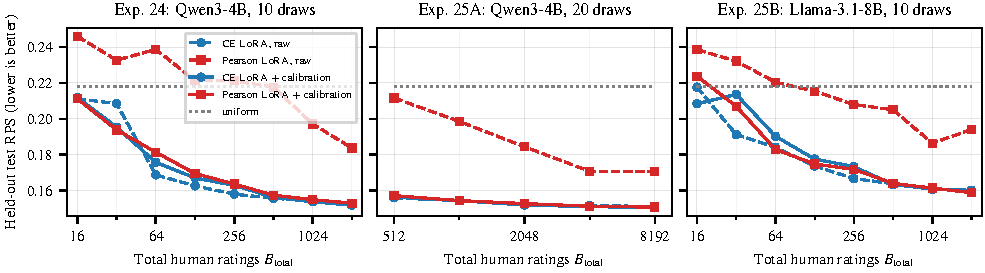
\includegraphics[width=\textwidth]{figures/fig_lora_helpsteer2.pdf}
\caption{\textbf{CE training is far better raw, but after an identical calibration the two objectives are statistically indistinguishable.}
LoRA judges on HelpSteer2 helpfulness: raw versus calibrated forecasts.
Vertical axis: held-out test RPS (0--1; lower is better); horizontal axis: total human ratings $B_{\mathrm{total}}$ split among training, validation and calibration.
Dashed: raw forecasts; solid: after an identical 7-parameter post-hoc calibration; blue: CE-trained; red: Pearson-trained; dotted: uniform.
Test data: 1{,}038 held-out responses from 519 held-out prompts; panels: experiment 24 (Qwen3-4B, 10 matched draws), experiment 25A (Qwen3-4B, up to 8{,}192 ratings, 20 draws) and experiment 25B (Llama-3.1-8B, 10 draws).
Human reference, leave-one-vote-out RPS: $0.14567$.
Both objectives use one optimizer, one schedule and the validation-RPS checkpoint rule; the correlation objective is not convex, so its curve reflects this optimizer, start and budget.}
\label{fig:lora-hs2}
\end{figure}

\subsection{Tables and figures that support the main text}
\label{app:extra-tables}

\Cref{tab:exp29} and \Cref{tab:scaling} give the numbers behind \Cref{fig:exp29} and \Cref{fig:scaling}; \Cref{fig:exp28-five} to \Cref{fig:ratings-needed} show curves that the main text summarizes in words.

\begin{table*}[t]
\caption{\textbf{The Pearson-trained judge is worse than the cross-entropy (CE)-trained judge in all seven setups, and the interval excludes zero in each.}
Four low-rank adaptation (LoRA) objectives at the largest budget (experiment 29).
Held-out test ranked probability score (RPS) of the raw forecasts (0--1; lower is better) of LoRA judges trained with CE, RPS, mean squared error (MSE) or Pearson correlation on $B$ total human ratings. One rating per item except where noted. Models: Qwen3-4B-Instruct-2507 or Llama-3.1-8B-Instruct. Ten nested training draws per budget.
The Pearson-trained judge has the highest raw RPS of the four objectives in six setups; on DICES with Llama-3.1-8B the MSE-trained judge is higher ($0.267$ against $0.251$).
``Pearson$-$CE'' is the test RPS of the Pearson-trained judge minus the test RPS of the CE-trained judge on the same held-out items; positive favors the CE-trained judge.
The band is a two-way crossed simultaneous max-$t$ 95\% band over budgets, from 4{,}000 paired cluster-bootstrap draws that resample training draws and held-out units together.
Every judge is trained by AdamW with a validation-RPS checkpoint; the Pearson objective is not convex, so the Pearson-trained row reflects this optimizer, start and budget.
$^{\ast}$The CE and Pearson HelpSteer2 runs are those of experiment 24; the RPS and MSE runs were added in experiment 29 on the same bundle and draws.}
\label{tab:exp29}
\centering\scriptsize
\begin{tabular}{lrrrrrrl}
\toprule
LoRA setup & $B$ & CE & RPS & MSE & Pearson & Pearson$-$CE & Crossed 95\% band \\
\midrule
ChaosNLI, Qwen3-4B & 2048 & 0.1490 & \textbf{0.1481} & 0.1521 & 0.1622 & +0.0132 & [+0.0063, +0.0202] \\
ChaosNLI, Llama-3.1-8B & 2048 & 0.1555 & \textbf{0.1548} & 0.1580 & 0.1898 & +0.0344 & [+0.0193, +0.0494] \\
ChaosNLI, 5/item, Qwen3-4B & 1280 & \textbf{0.1530} & 0.1560 & 0.1646 & 0.1910 & +0.0379 & [+0.0216, +0.0543] \\
alphaNLI ($K{=}2$), Qwen3-4B & 1024 & \textbf{0.1862} & 0.1873 & 0.1866 & 0.2082 & +0.0220 & [+0.0117, +0.0322] \\
DICES, Qwen3-4B & 1024 & \textbf{0.2088} & 0.2101 & 0.2638 & 0.2849 & +0.0761 & [+0.0572, +0.0950] \\
DICES, Llama-3.1-8B & 1024 & \textbf{0.2060} & 0.2061 & 0.2666 & 0.2505 & +0.0445 & [+0.0191, +0.0700] \\
HelpSteer2$^{\ast}$, Qwen3-4B & 2048 & \textbf{0.1521} & 0.1527 & 0.1827 & 0.1838 & +0.0316 & [+0.0187, +0.0445] \\
\bottomrule
\end{tabular}

\end{table*}

\begin{table*}[t]
\caption{\textbf{Every cross-entropy (CE) curve has a fitted exponent between $0.33$ and $0.89$, while no Pearson curve in ranked probability score (RPS) is a power law.}
Scaling-law fits and verdicts (experiment 31).
Held-out test RPS (0--1; lower is better) at the largest number of human ratings $N_{\max}$ tested, for the CE-fit (or CE-trained) and the Pearson-fit (or Pearson-trained) judge. Frozen-judge panels are means over five frontier judges with one rating per item. Low-rank adaptation (LoRA) panels are raw forecasts with ten draws per budget.
The CE-fit floor and exponent $b$ come from the weighted fit of Equation~\eqref{eq:scaling} with percentile 95\% intervals from 2{,}000 parametric bootstrap draws.
``Floor not identified'' means the floor's interval is wider than the curve's range, and ``poor power-law fit'' that the root-mean-square residual exceeds 10\% of the range.
Judges are chosen as in \Cref{fig:scaling}; exhaustive search for the head, AdamW with a validation checkpoint for LoRA.}
\label{tab:scaling}
\centering\scriptsize
\setlength{\tabcolsep}{3pt}
\begin{tabular}{lrrrccl}
\toprule
Panel (held-out test RPS) & $N_{\max}$ & CE-fit at $N_{\max}$ & Pearson-fit at $N_{\max}$ & CE-fit floor [95\%] & CE-fit $b$ [95\%] & Pearson-fit curve (experiment 31 verdict) \\
\midrule
Exp.\ 28, ChaosNLI SNLI & 256 & 0.115 & 0.134 & 0.105 [0.000, 0.118] & 0.33 [0.04, 0.86] & slow decline, floor not identified \\
Exp.\ 28, ChaosNLI MNLI-m & 256 & 0.163 & 0.185 & 0.160 [0.147, 0.165] & 0.64 [0.28, 1.09] & slow decline, floor not identified \\
Exp.\ 28, alphaNLI (two classes) & 256 & 0.120 & 0.125 & 0.115 [0.000, 0.126] & 0.54 [0.05, 1.64] & slow decline, floor not identified \\
Exp.\ 28, DICES-350 & 256 & 0.226 & 0.276 & 0.221 [0.180, 0.231] & 0.60 [0.18, 1.13] & slow decline, floor not identified \\
Exp.\ 28, DICES-990 & 256 & 0.198 & 0.261 & 0.192 [0.159, 0.201] & 0.58 [0.21, 0.99] & flat \\
Exp.\ 29, ChaosNLI, Qwen3-4B & 2048 & 0.149 & 0.162 & 0.148 [0.146, 0.149] & 0.89 [0.76, 0.99] & slow decline, floor not identified \\
Exp.\ 29, ChaosNLI, Llama-3.1-8B & 2048 & 0.155 & 0.190 & 0.151 [0.146, 0.154] & 0.64 [0.49, 0.78] & poor power-law fit \\
Exp.\ 29, alphaNLI, Qwen3-4B & 1024 & 0.186 & 0.208 & 0.179 [0.117, 0.184] & 0.56 [0.13, 0.92] & poor power-law fit \\
Exp.\ 29, DICES, Qwen3-4B & 1024 & 0.209 & 0.285 & 0.204 [0.196, 0.208] & 0.71 [0.46, 0.96] & flat \\
Exp.\ 29, DICES, Llama-3.1-8B & 1024 & 0.206 & 0.251 & 0.203 [0.194, 0.206] & 0.89 [0.50, 1.29] & poor power-law fit \\
Exp.\ 29, HelpSteer2, Qwen3-4B & 2048 & 0.152 & 0.184 & 0.151 [0.149, 0.152] & 0.76 [0.64, 0.89] & slow decline, floor not identified \\
\bottomrule
\end{tabular}

\end{table*}

\begin{figure}[t]
\centering
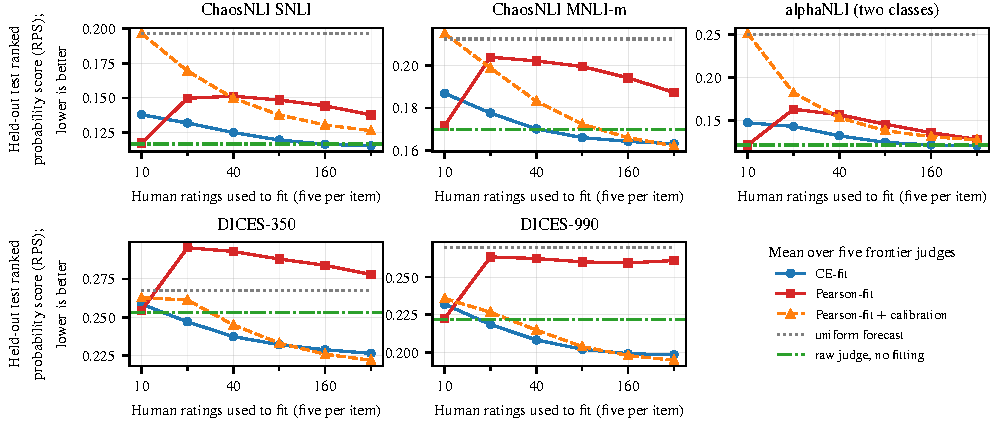
\includegraphics[width=0.92\textwidth]{figures/fig_exp28_five_per_item.pdf}
\caption{\textbf{In every set the Pearson-fit curve is worse at 20 ratings than at 10 and stays above the raw judge at every larger budget, while the CE-fit curve falls at every step.}
Frozen frontier judges with five ratings per item (experiment 28).
Vertical axis: held-out test RPS (0--1; lower is better), mean over five frontier judges; horizontal axis: human ratings used to fit, 10 to 320 (2 to 64 items with five ratings each; log scale).
Data: ChaosNLI SNLI (600 items), MNLI-matched (600), alphaNLI (400; two classes), DICES-350 (350) and DICES-990 (400 items); each held-out item is scored against all of its collected labels.
CE-fit minimizes, and Pearson-fit maximizes, its objective on the training ratings over 27 calibration settings of the judge's own probabilities, by exhaustive search; Pearson-fit + calibration follows the Pearson-chosen setting with four quantile-bin category frequencies (0.5 pseudo-count) fitted on the same training ratings.
Each point averages 200 draws; no interval is drawn here, and the break-even budgets of \Cref{tab:exp28} come from simultaneous one-sided 97.5\% bounds.}
\label{fig:exp28-five}
\end{figure}

\begin{figure}[t]
\centering
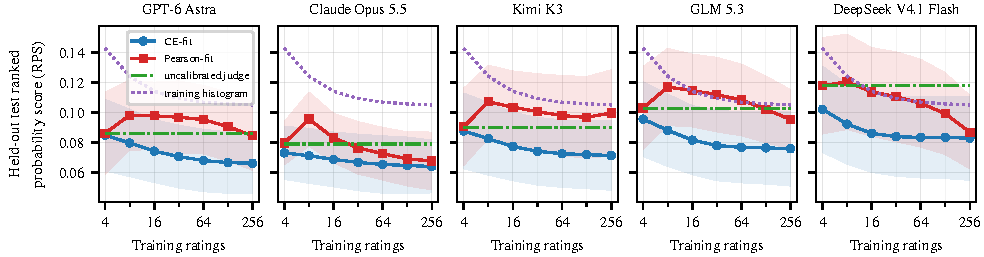
\includegraphics[width=\textwidth]{figures/fig_exp26_per_judge.pdf}
\caption{\textbf{The CE-fit curve lies below the Pearson-fit curve in all 35 judge-by-budget cells, but the bands overlap everywhere, so the figure supports the ranking and does not identify any law.}
Five frontier judges on fresh homework (experiment 26).
Vertical axis: held-out test RPS (0--1; lower is better) on 16 held-out answers per fold, scored against two grader scores each; horizontal axis: training ratings, 4 to 256, two per answer (log scale).
Data: 160 short answers of 67 questions in ten homework folds, each fold held out once; the lines are means over folds and 200 training draws.
Shaded bands are 95\% two-sided overlap-adjusted $t$ intervals over the ten folds (standard deviation times $\sqrt{1/10+1/9}$, 9 degrees of freedom) for the CE-fit and Pearson-fit judges.
CE-fit and Pearson-fit choose among 27 calibration settings of each judge's six grade probabilities by exhaustive search on the training ratings.}
\label{fig:exp26}
\end{figure}

\begin{figure}[t]
\centering
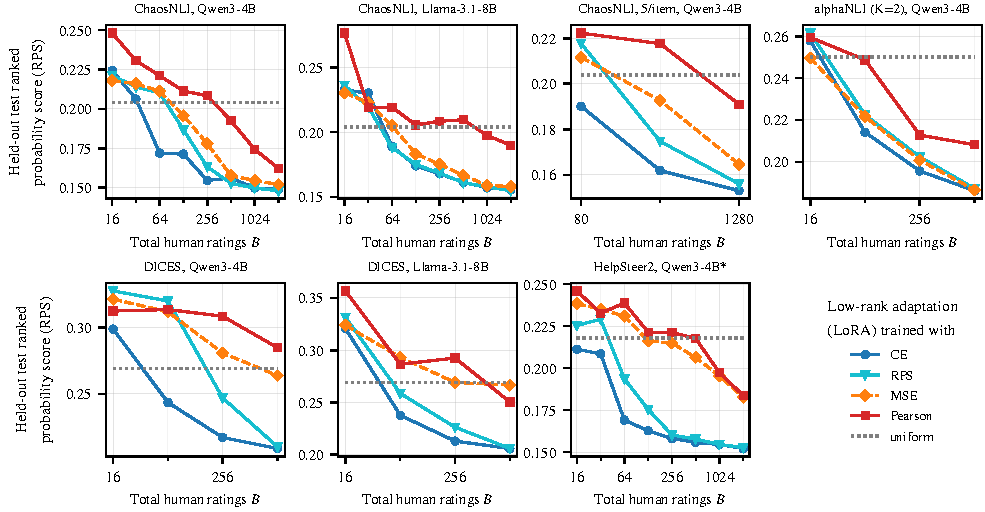
\includegraphics[width=\textwidth]{figures/fig_exp29_curves.pdf}
\caption{\textbf{CE and RPS training track each other, squared error follows them at $K=2$ and falls behind at $K\ge3$, and the Pearson-trained curve lies above the CE curve at nearly every budget.}
Learning curves of four LoRA objectives (experiment 29).
Vertical axis: held-out test RPS (0--1; lower is better) of raw forecasts; horizontal axis: total human ratings $B$ used for training (log scale), one rating per item unless the panel says five per item.
LoRA of Qwen3-4B-Instruct-2507 or Llama-3.1-8B-Instruct on ChaosNLI, alphaNLI (two classes), DICES and HelpSteer2 (CE and Pearson from experiment 24); each point is a mean over ten nested training draws, and no band is drawn (bands for the largest budget are in \Cref{tab:exp29}).
Each objective uses one optimizer, one schedule and the same validation-RPS checkpoint rule; the correlation objective is not convex, so it reflects this optimizer, start and budget.}
\label{fig:exp29-curves}
\end{figure}

\begin{figure}[t]
\centering
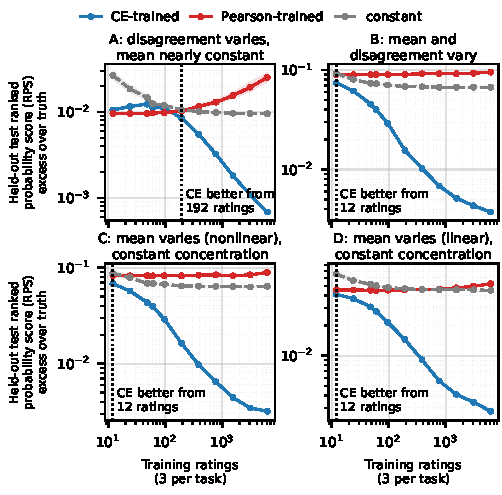
\includegraphics[width=0.56\textwidth]{figures/fig_ratings_needed.pdf}
\caption{\textbf{The CE-trained judge wins from 12 ratings where the mean carries the signal (B, C, D) and needs 192 ratings only in A, where the mean says little.}
Ratings needed in four synthetic scenarios (experiment 08).
Vertical axis: held-out test RPS excess over the true distribution, that is the RPS of the judge's forecast minus the RPS of the true conditional distribution on 500 fresh tasks (lower is better; log scale); horizontal axis: training ratings, three per task.
Targets are beta-binomial distributions over six ratings: A has an almost constant mean and varying disagreement, B a nonlinear mean and varying disagreement, C a nonlinear mean and constant concentration, D a linear mean and constant concentration.
The judge is a softmax over a linear map of 13 features, trained by L-BFGS-B (400 iterations) from the training histogram with a fixed ridge; the CE objective is convex and the Pearson objective is not, so the Pearson curve reflects this optimizer and start.
Lines are means over 100 seeds with 95\% percentile bootstrap bands (10{,}000 draws); the dotted line marks the smallest budget from which the paired difference (Pearson-trained minus CE-trained) has a lower bound above zero at every larger budget.}
\label{fig:ratings-needed}
\end{figure}

\clearpage

\section{Provenance, reproduction and data handling}
\label{app:provenance}

\paragraph{Source and build.}
This memo was built from the repository \url{https://github.com/brando90/judges-dont-need-psychometrics-or-corr} on 11-25-2026.
Every experiment result it reads was committed at or before commit \texttt{2bd73d9}, and the memo's own files are in the commit that carries this PDF.
They sit in \texttt{paper\_latex\_and\_notes/ICML\_format\_tech\_memo\_11-25-2026/}.
Running \texttt{python3 -I make\_memo\_assets.py} there regenerates every figure and table of this memo from committed result files and writes \texttt{assets\_log.txt}; \texttt{make} then runs \texttt{pdflatex} and \texttt{bibtex}.
Neither step calls a model.

\paragraph{Where each number comes from.}
We typed each number in the text from a result file or script output committed under \texttt{experiments/}, or from the log of \texttt{make\_memo\_assets.py}, and \texttt{check\_numbers.py} compares them with those sources.
The checker is a screening aid: it accepts a number that appears anywhere in the sources and does not confirm what the number refers to.
\Cref{tab:index} names the folder of each experiment; the folders hold the frozen protocol, the run receipts, request hashes and a reading guide that states which data, metric and comparison each number uses.

\paragraph{Data.}
Public sets (ChaosNLI, DICES, HelpSteer2, KonIQ-10k, SummEval, USR, MovieLens-100K) are used as released.
The retrospective theorem-judge studies use 75 artifacts, 25 tasks and 195 expert ratings, and the homework studies use 160 short answers with two graders; this memo reports only aggregate results from them and reproduces no rater identity and no raw rating.
No new human ratings were collected for the memo.

\paragraph{Prior exposure and the human floor.}
Results on the 75 theorem artifacts are not fresh: experiments 02, 09, 10, 12, 14, 16, 18, 19 and 20 reuse them (Section~\ref{sec:limits}).
The per-item vote counts that a human leave-one-vote-out floor needs for the frozen-judge panels are not saved in the repository, so the memo estimates no such floor; it quotes the reference scores that experiment 29 saved for its test sets as descriptive values.

\paragraph{Cost.}
The scaling-law analysis of experiment 31, the figures and the tables of this memo are free CPU computations on saved results.
The model calls of the underlying experiments (frontier-judge queries through the Stanford AI API Gateway, LoRA training of Qwen3-4B-Instruct-2507 and Llama-3.1-8B-Instruct) are described in the folders of experiments 21, 26, 28 and 29.

\paragraph{Related deposit.}
The identification results of Section~\ref{sec:identification} were deposited as a frozen preprint in the Stanford Digital Repository~\citep{miranda2026correlation}; this memo extends them with proofs, controlled studies, matched-budget comparisons and scaling fits.


\end{document}
